
\chapter{UNH TABLESAT 1A}
\label{chap:UNHTableSat1A}

The UNH TableSat 1A is a limited 3-DOF experimental test bed analog for the NASA MMS satellite (Figure \ref{fig:TSatFullView}).  All electronics, booms, and actuators are attached to a circular PVC deck.  The aluminum hub at its center has a hollow center which allow it to rest on a center post giving the deck full rotation about its z-axis and limited rotations about its x and y-axes.  Five out of the six booms present on the MMS spacecraft are represented on TableSat 1A.  The four SDP booms extend radially from the deck at 90 degree intervals.  One of the MMS's ADP booms is modeled with a boom attached to the center post of the TableSat.

\begin{figure}[H]
\centerline{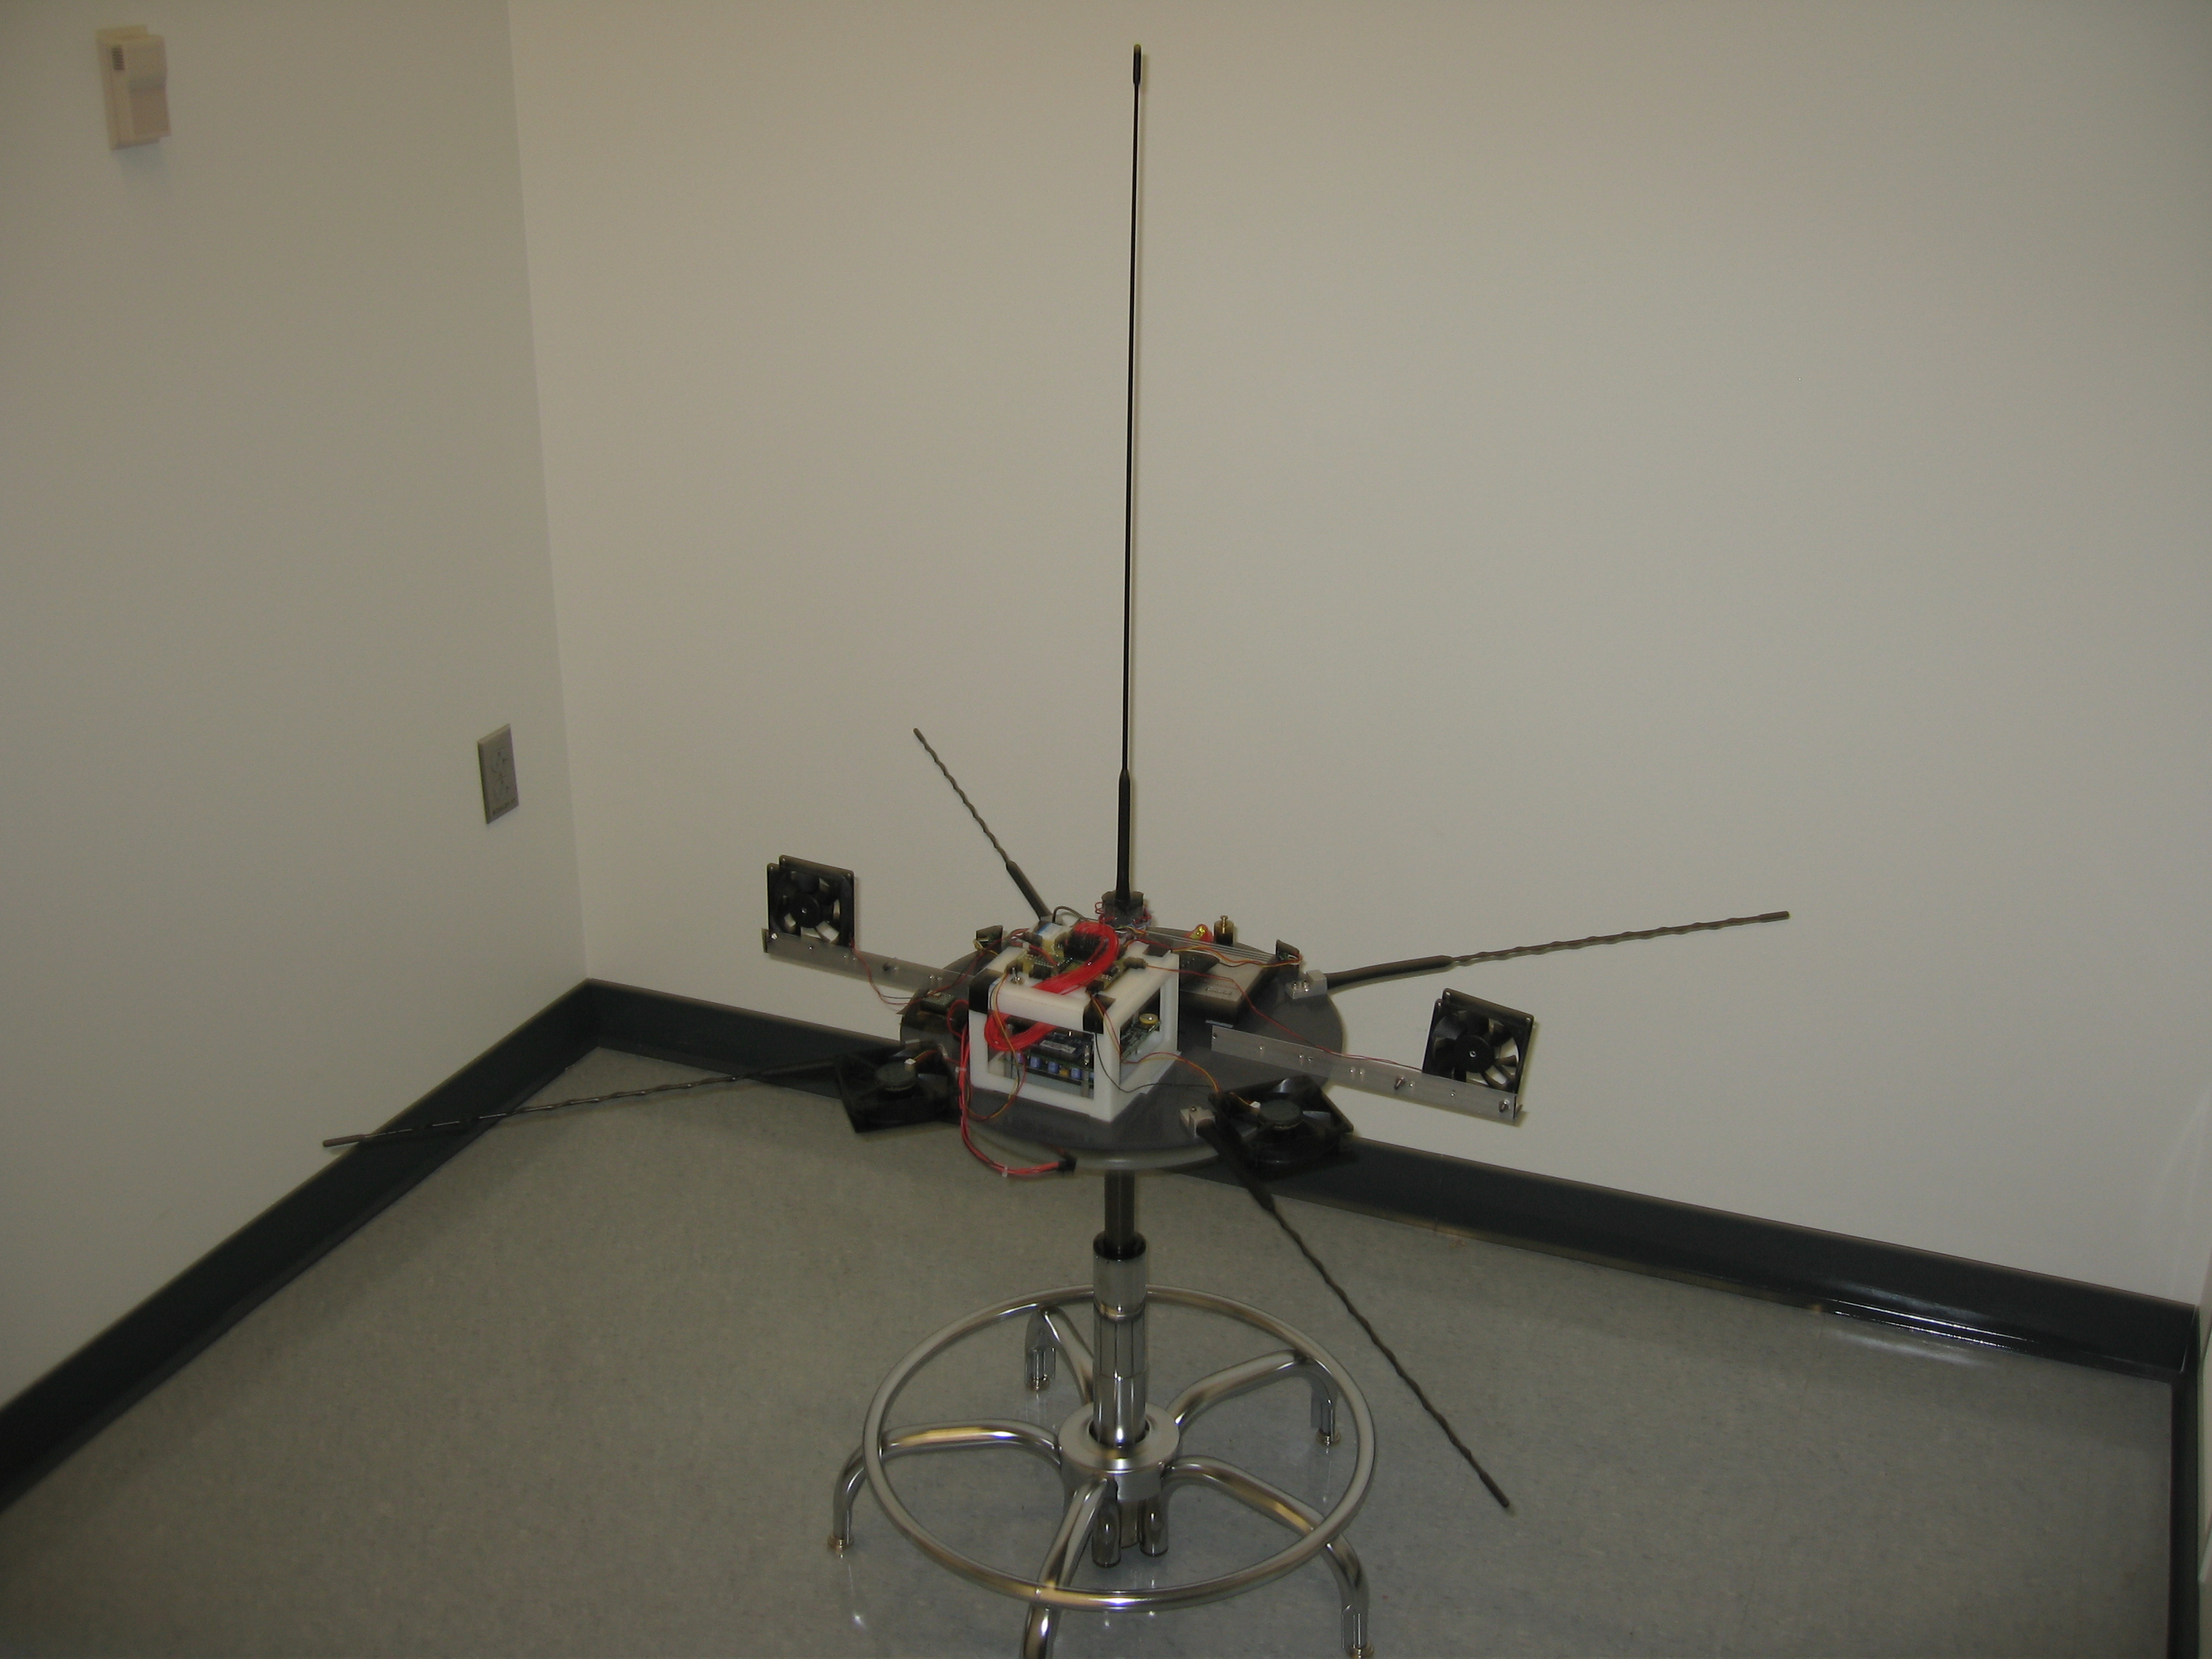
\psfig{file=figures/tsat_full_view.eps,height=3in}}
\caption{TableSat 1A Full View}
\label{fig:TSatFullView}
\end{figure}

\section{Booms}
\label{sec:Booms}

The ADP booms were modeled with a selection of flexible antenna.  Attaching weights to the tip and varying the stiffness of the selected antenna allowed for some tuning to the fundamental frequency of the booms.  Since the SDP booms extend perpendicularly to gravity, two choices were made for their modeling.  For free motion, the cylindrical antenna for the ADP boom were also used for the SDP booms.  The disadvantage to these booms especially when adding weights to reduce their natural frequency was that they would droop under the gravitational pull.  An alternative to the cylindrical antenna for the SPD booms were thin and flat strips of metal.  Attaching them to the TableSat's deck such that they were standing on edge removed the gravitational drooping since the booms, but still allowed for the boom to bend back and forth in the spin plane.  This also restricted the boom's freedom of movement, so a combination of results would be needed to get a better idea of how the MMS booms would react in orbit.

\begin{figure}[H]
\centerline{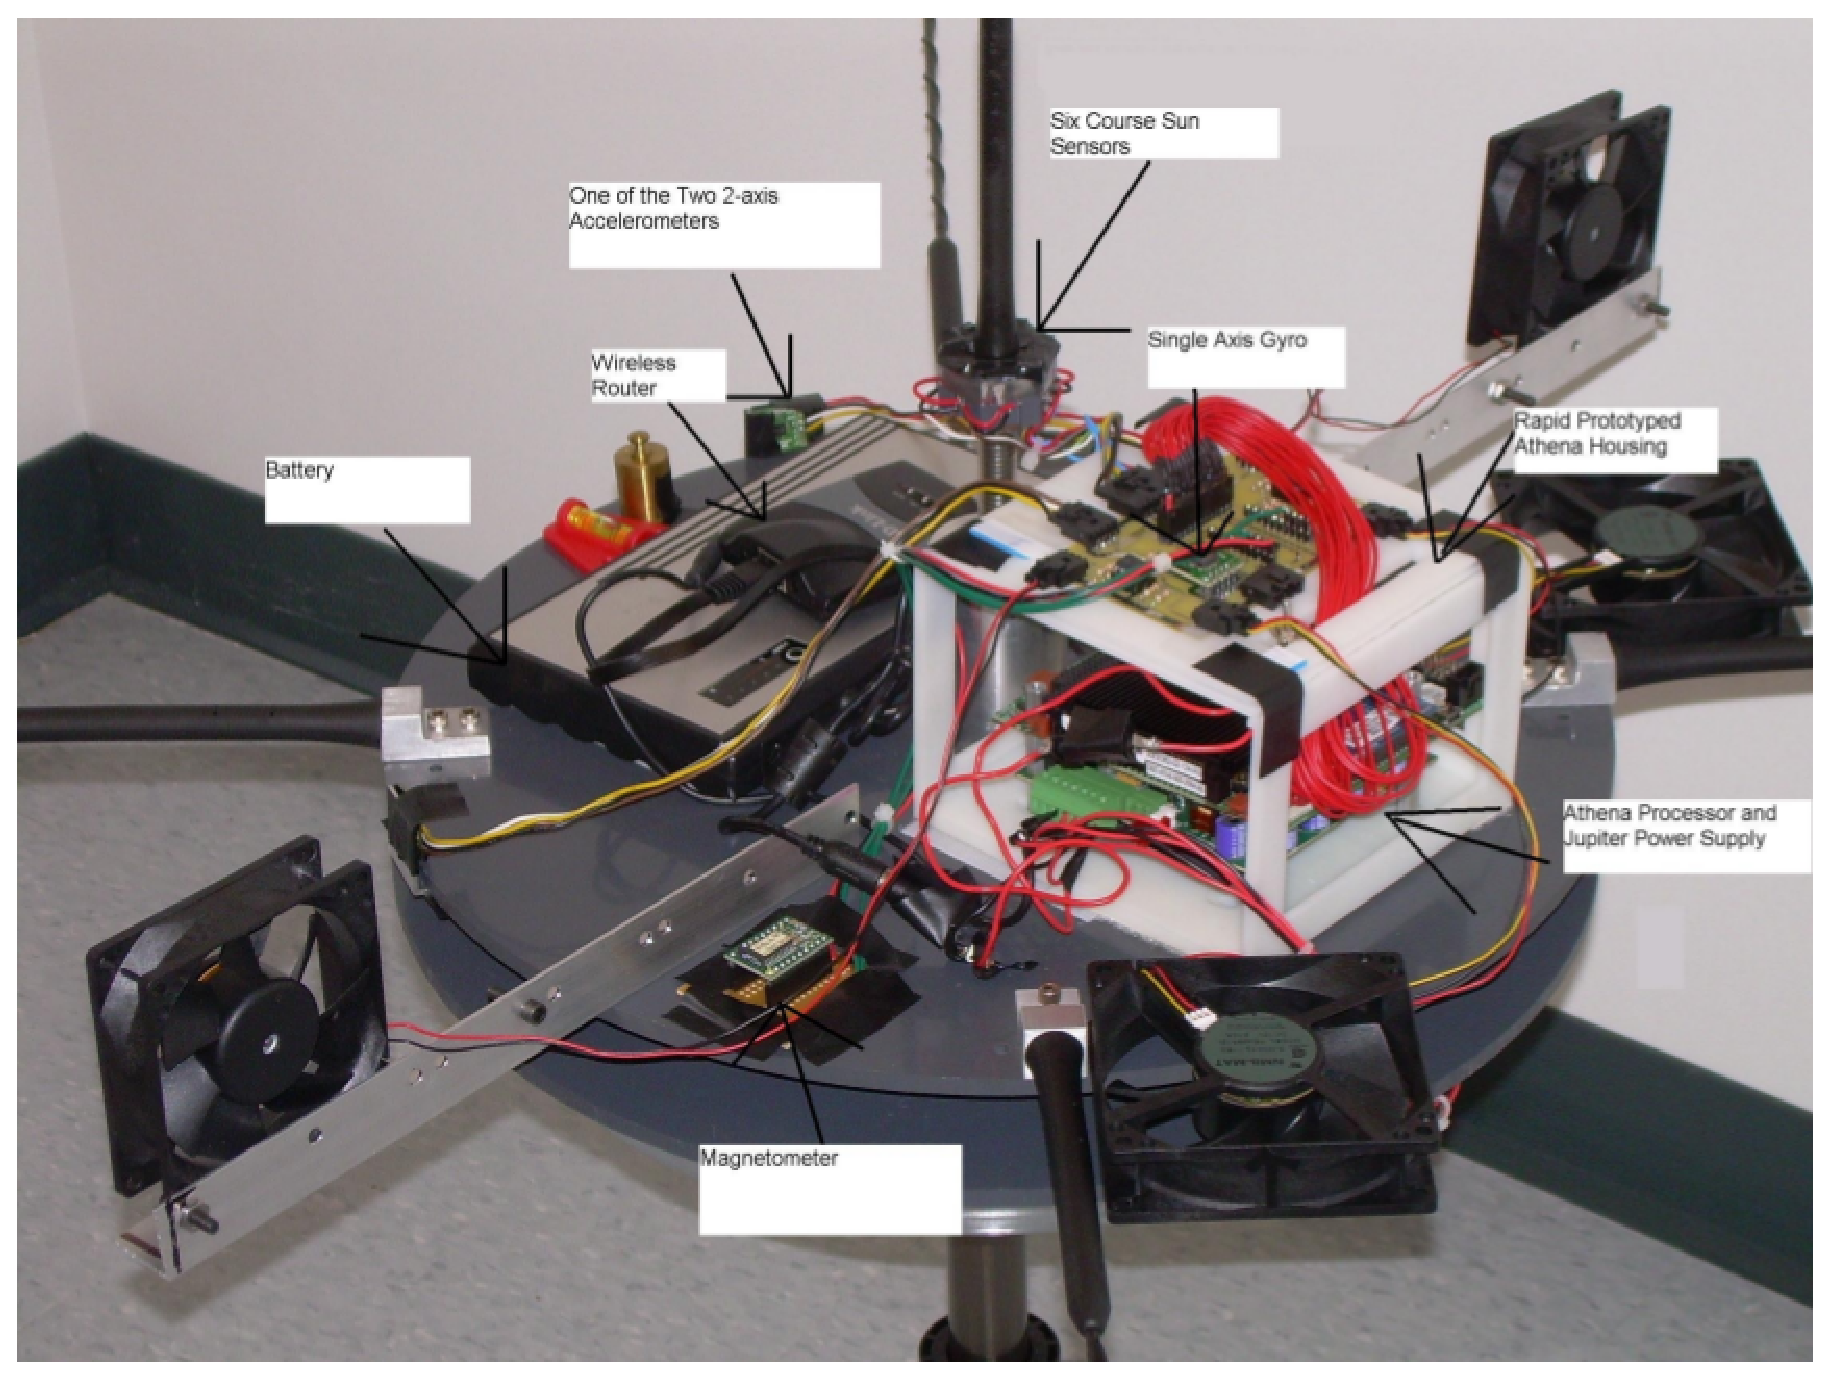
\psfig{file=figures/tsat_components.eps,height=4in}}
\caption{TableSat Components}
\label{fig:TSatComponents}
\end{figure}

\section{Flight Controller}
\label{sec:FlightController}

The onboard flight controller was an Athena PC from Diamond Systems powered by a Jupiter power supply and lithium-ion rechargeable battery.  The Athena processor and Jupiter power supply were mounted in a rapid prototyping housing with open sides for ventilation.  A custom printed circuit board designed by Jeff Kite \TODO{need footnote reference here?} was mounted on top of the rapid prototyping housing.  User Datagram Protocol (UDP) communication (Section \ref{subsec:MessageDefinitions}) to the base station is transmitted through a wireless access point.

\TODO{forgot cs student's name} created a C program based off of Vess' ``open-loop'' flight controller \cite{vessthesis} .  This program is responsible for listening to a UDP socket on the TableSat and performing a limited set of actions based on the message packets received from the base station.  The most common messages triggered actions like altering the voltages applied to the actuators, and scanning the sensor ports and sending the voltages back to the base station through UDP.

\section{Actuators}
\label{sec:Actuators}

In addition to the booms extending from the TableSat's deck, four single direction analog input computer fans were mounted to provide a source of thrust (Figure \ref{fig:TSatComponents}).  Two fans were mounted standing upright to provide radial torque.  One pointing clockwise and the other counter clockwise had their centers level with the pivot point inside the central hub and provided control of the rotation rate.  Two other fans were mounted facing down to provide limited opportunities for nutation control.

Section \ref{subsec:MessageDefinitions} defines message number 18 as the method for communicating with the TableSat to specify the voltage to apply to each of the individual fans.  Voltages are set through an analog port and are allowed to vary between \TODO{find limits}.  Voltages below \TODO{Lower limit} either are not high enough to overcome the static friction, or risk damaging the fan by rotating far below the normal speed.

\TODO{CO2 thrusters}

\section{Sensors}
\label{sec:Sensors}

Four classes of analog sensors were implemented in TableSat 1A's design. Gyroscope (Section \ref{subsec:Gyroscope}) and accelerometer (Section \ref{subsec:Accelerometer}) for velocity measurements.  Course sun sensor (Section \ref{subsec:CourseSunSensor}), and magnetometer (Section \ref{subsec:TripleAxisMagnetometer}) for position measurements.  These sensors and the four actuators filled all available analog ports on the onboard Athena flight computer.  As is described below, the gyroscopes and accelerometers were not used for the observer-based controllers in this thesis leaving just positional measurements from the course sun sensors and triple axis magnetometer.

\begin{figure}[H]
\centerline{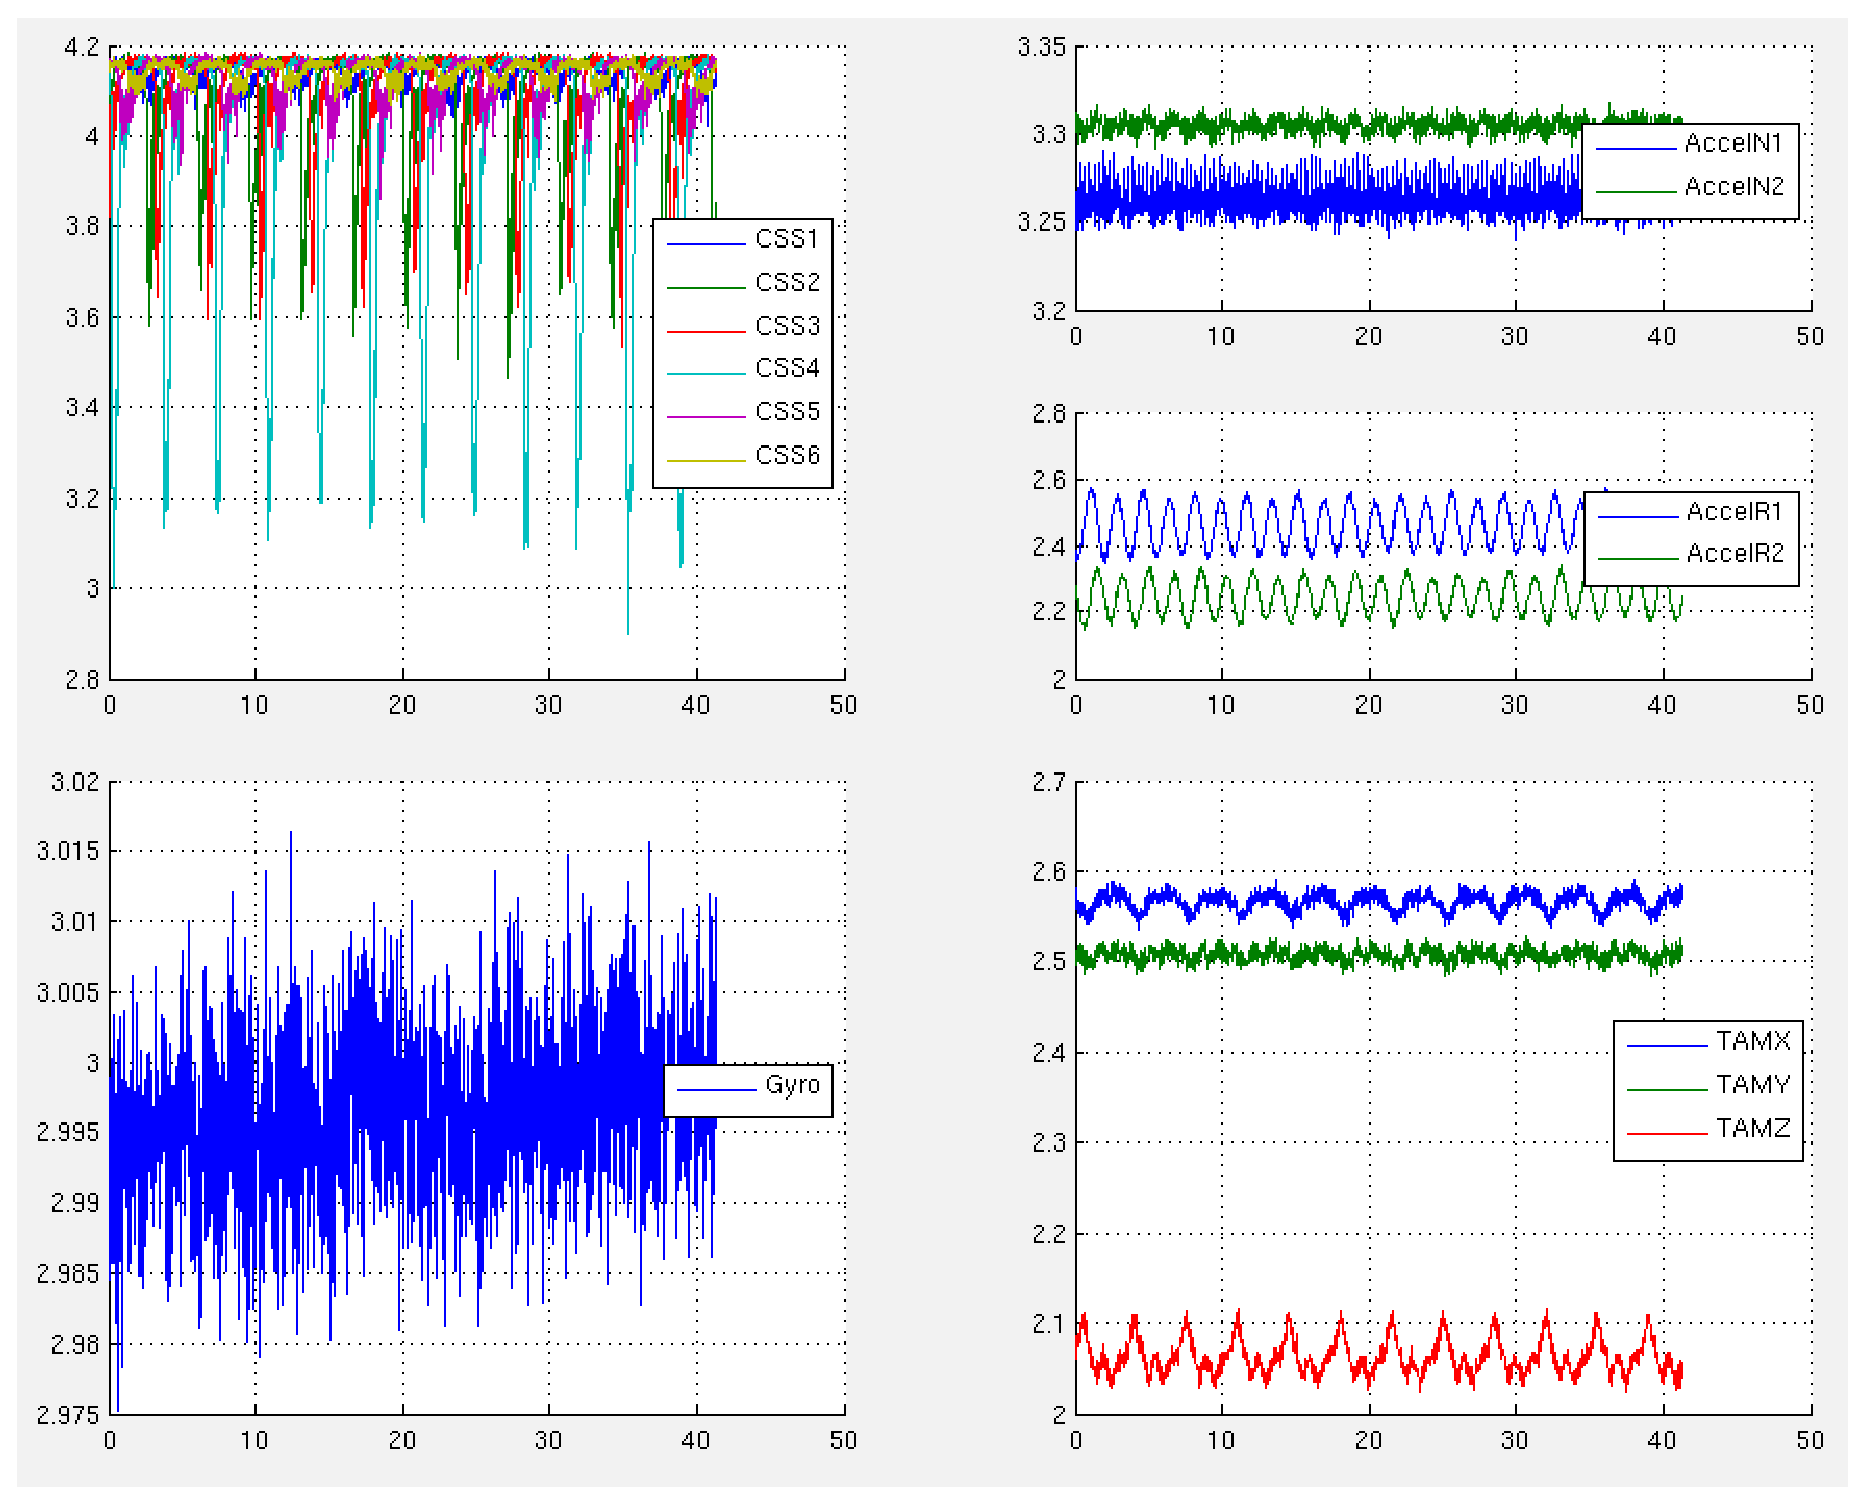
\psfig{file=figures/sensor_voltage_charts.eps,height=4in}}
\caption{Sensor Voltage Readings}
\label{fig:SensorVoltageReadings}
\end{figure}

\subsection{Gyroscope}
\label{subsec:Gyroscope}

Gyroscopes remain one of the most accurate sensors for detecting changes to a structure's angular body rates.  The issue with their use is that to increasing the accuracy of a gyroscope means using a heavier sensor.  Since any additional weight is a serious launch concern for a satellite, this research for NASA's MMS mission uses the gyro scope solely as a verification method.  The gyroscope selected for TableSat 1A is a single axis gyroscope that is mounted on the printed circuit board at the top of the flight controller housing.  The gyroscope is oriented to detect changes in body rates about the TableSat's z-axis although is mounted slightly above the center hub's pivot point so will pick up small signals from any limited nutation encountered.

\subsection{Accelerometer}
\label{subsec:Accelerometer}

Two 2-axis accelerometers are mounted at the circumference or TableSat's deck.  The accelerometers are oriented such that one signal detects vertical acceleration with a 2g resolution and the other a radial signal with a 0.5g resolution.  The rotational accelerometers ended up picking up a small signal which is either due to oscillations in angular velocity or a nutation subjecting the radial accelerometer to gravitational effects.  The vertical components of the accelerometers had such low signal to noise ratios that heavy filtering would be required to even attempt to detect the out of plane rotations.  Any significant nutations allowed by the limited 3-DOF design would damp out quickly enough to be eliminated before the filtering could identify the signal.  Given these severe limitations in the sensor's measurements, for the purpose of this thesis the accelerometer measurements are ignored.

\subsection{Course Sun Sensor}
\label{subsec:CourseSunSensor}

The course sun sensor (CSS) for UNH TableSat 1A was constructed from a hexagonal piece of PVC pipe with a photodiode mounted in each face (Figure \ref{fig:CSS}).  Photodiodes are light detectors that convert captured light to electricity.  Given the inability to use the gyroscope and the accelerometer's high level of noise, the course sun sensor proved to be the most reliable sensor, but was limited to measuring a single value from the state matrix corresponding to rotations about the z-axis.  Each photo diode detected light level in its field of view and would generate a voltage generally proportional to that value.  The photodiodes are mounted above the center hub and faced out around the spin plane.  By placing a single light source in a dark room, the course sun sensor's voltages could be used to calculate the angular displacement about the body's z-axis.


\begin{figure}[H]
\centerline{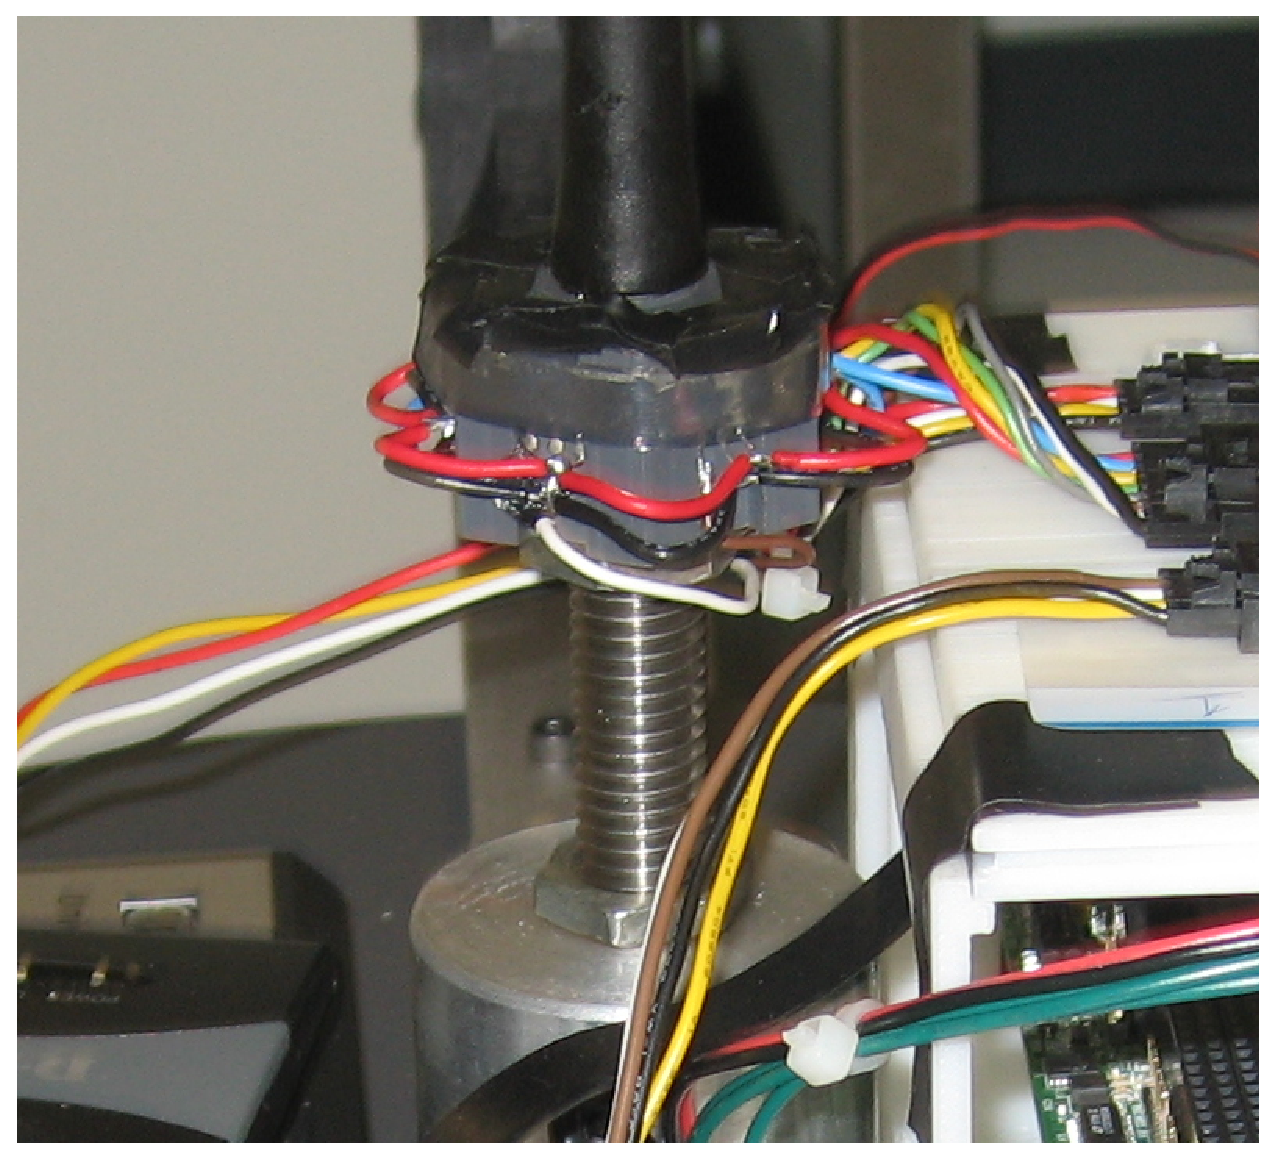
\psfig{file=figures/css.eps,height=2in}}
\caption{Course Sun Sensor Configuration}
\label{fig:CSS}
\end{figure}

Calculating the angular displacement about the body's z-axis is done using a method similar to a resultant force calculation.  Assuming all of the photodiodes volts per lumen rates are consistent, the voltages can be described as an equivalent force it the direction of the photodiode face.  Each force is decomposed into x and y components and then summed into a resultant force vector who's angle is used to represent the angular displacement of the TableSat.  Even though this method is fairly simplistic and that individual sensor voltage readings contained a moderate level of noise, this method proved to generate a very reliable and clean signal before even using filtering and estimation techniques.

\begin{subequations}
  \begin{align}
    V_{css\_x} & = \sum\limits_{i=1}^6 (V_{css\_x} - V_{css\_base}) \cos \left( \frac{2\pi}{6} (i-1)\right) \\
    V_{css\_y} & = \sum\limits_{i=1}^6 (V_{css\_x} - V_{css\_base}) \sin \left( \frac{2\pi}{6} (i-1)\right) \\
    \psi & = \tan^{-1} \frac{V_{css\_y}}{V_{css\_x}}
  \end{align}
  \label{eqn:CSSResultantForce}
\end{subequations}

\begin{figure}[H]
\centerline{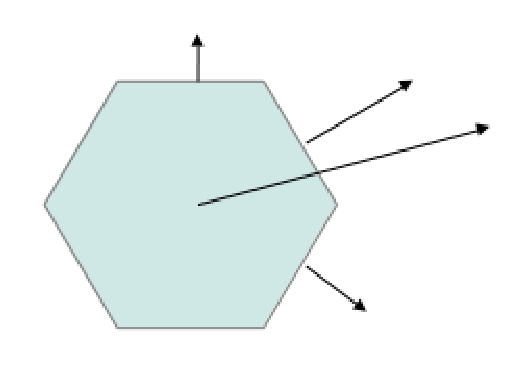
\psfig{file=figures/css_vectors.eps,height=1in}}
\caption{Photodiode Resultant Force Calculation for Yaw}
\label{fig:CSSVectors}
\end{figure}


\subsection{Triple Axis Magnetometer}
\label{subsec:TripleAxisMagnetometer}

Along with the course sun sensor, the triple-axis magnetometer (TAM) is used to measure position.  The primary advantage to the TAM over the course sun sensor it that it measures the full position state rather than just position about the z-axis.  As seen in Figure \ref{fig:SensorVoltageReadings}, three voltages are reported to designate the TableSat's attitude.  Each voltage corresponds to the strength of the magnetic field in each orthogonal direction.  To determine a method of converting raw TAM voltages to a TableSat, the clockwise actuator was set to provide a constant thrust.  With the fraction of the pivot point, the system slowly stabilized to a relatively constant spin rate.  Once stabilized, TAM voltage readings were recorded at a rate of 50 Hz and written to a log.  The mean values were subtracted from each of the three axes and plotted (Figure \ref{fig:TAMRaw}).

\begin{figure}[H]
\centerline{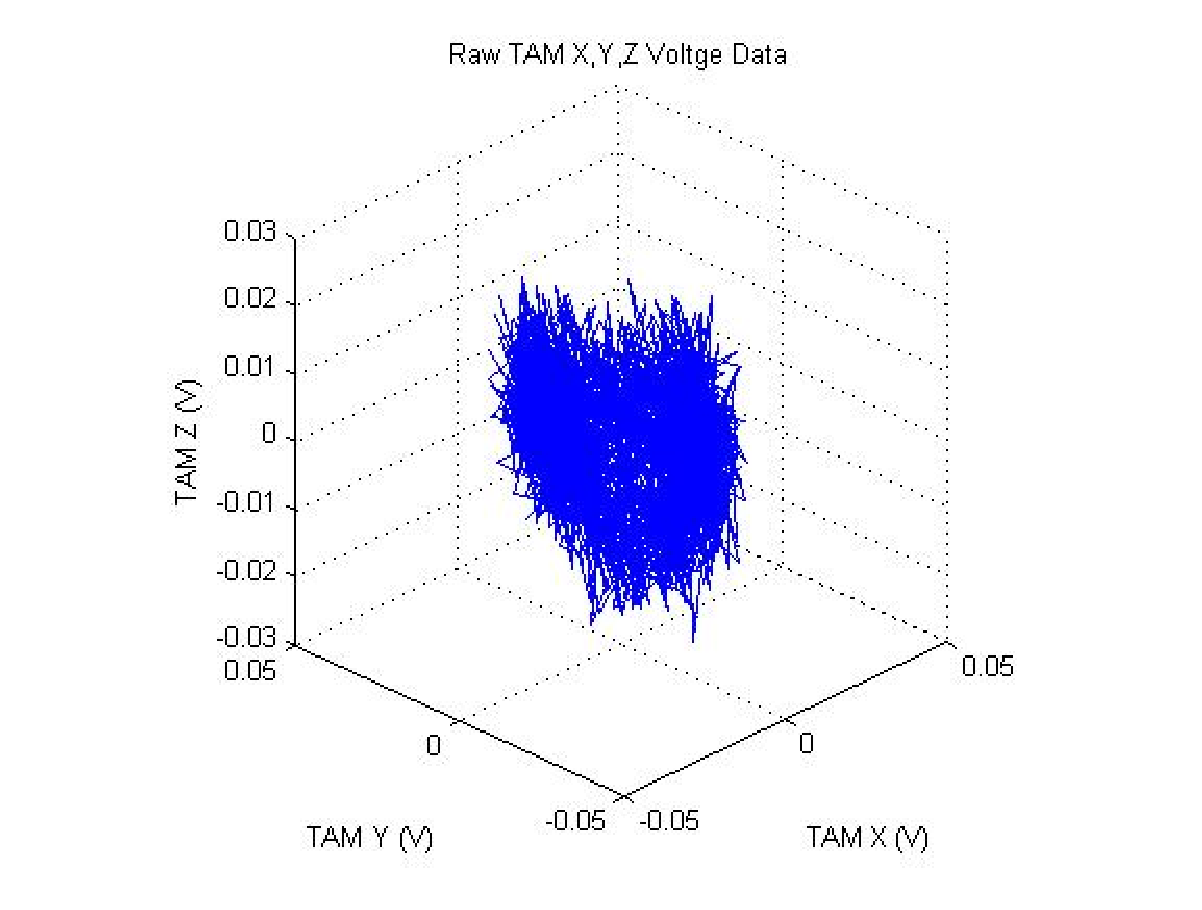
\psfig{file=figures/tam_raw.eps,height=4in}}
\caption{Raw TAM Voltages}
\label{fig:TAMRaw}
\end{figure}

Besides the slightly less dense center, the raw TAM measurements amount to a blob of points with no clear pattern.  If the signal is strong enough, a consistent path should be present.  Given the high sampling rate, aggressive filtering should be able to pull a signal out of the blob of data points.  A basic 40 point moving average was used as a first pass analysis to verify there is a signal in the data (Eq \ref{eqn:TAMMovingAvg}).  The moving average smoothed data is show in Figure \ref{fig:TAMMovingAverage}.  The good news being that a distinct an repeatable signal occurs as TableSat completes successive rotations.  The bad news is the irregular path that the magnetometer readings follow.

\begin{equation}
  x_i = \frac{1}{40} \sum^{39}_{j=0} x_{i-j}
  \label{eqn:TAMMovingAvg}
\end{equation}

\begin{figure}
  \begin{subfigure}[h!]{0.5\textwidth}
    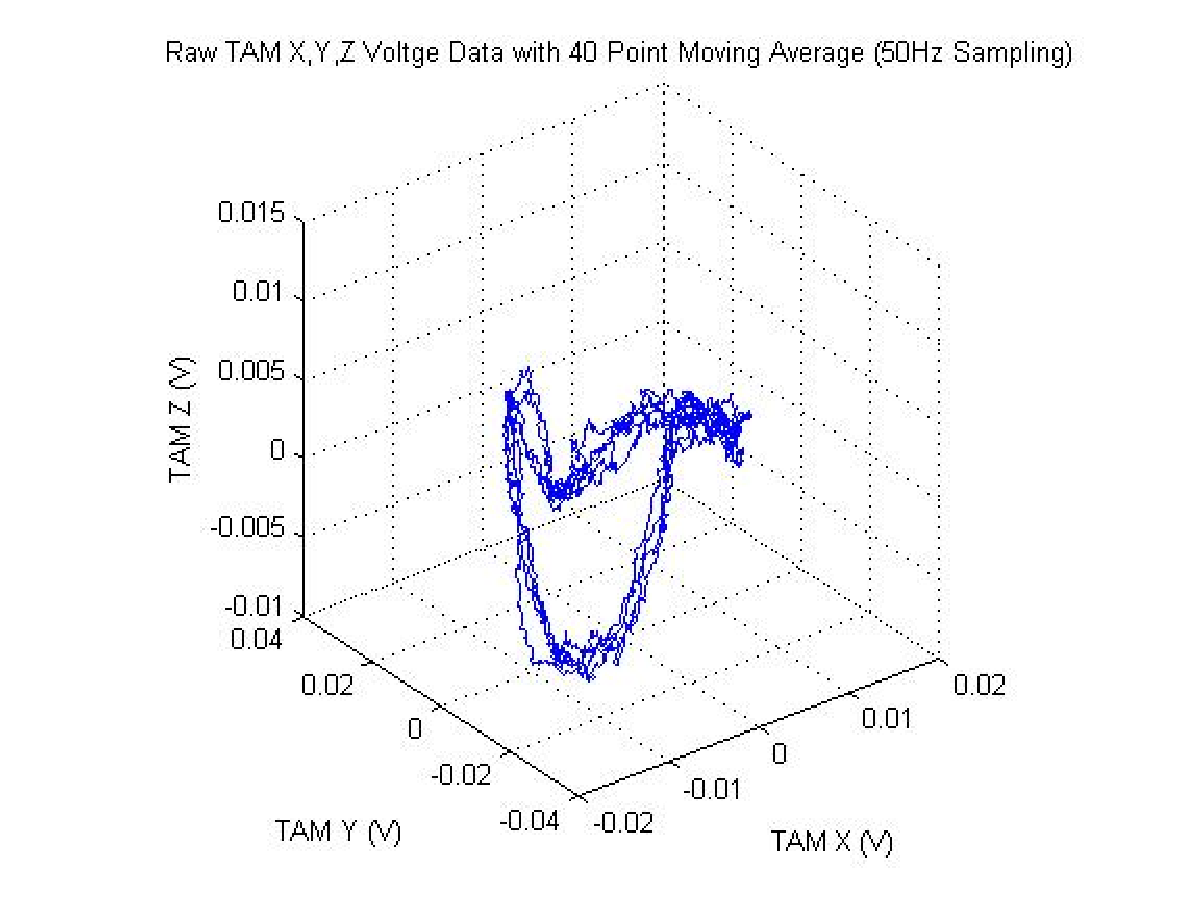
\includegraphics[width=\textwidth]{figures/tam_moving_average.eps}
    \caption{Raw TAM Voltages - Moving Average}
    \label{fig:TAMMovingAverage}
  \end{subfigure}
  ~
  \begin{subfigure}[h!]{0.5\textwidth}
    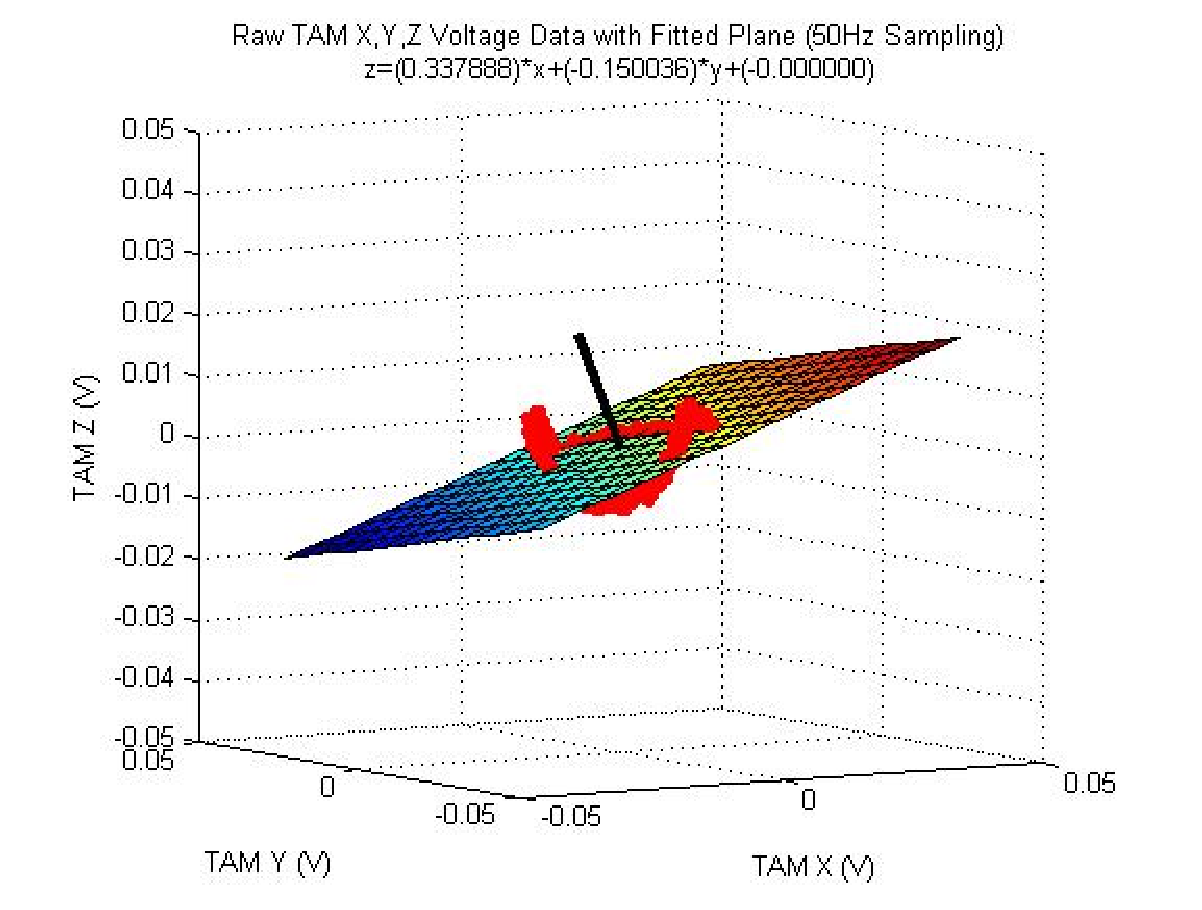
\includegraphics[width=\textwidth]{figures/tam_fitted_plane.eps}
    \caption{TAM Voltages with Fitted Plane}
    \label{fig:TAMFittedPlane}
  \end{subfigure}
  \caption{Determining Attitude from TAM}
  \label{fig:TAMSignal}
\end{figure}

Figure \ref{fig:TAMFittedPlane} shows the result of fitting a plane to the moving average smoothed TAM voltages.  The error in the fit between the smoothed TAM data points and the planar fit were too large to have much confidence in using this measure for nutation detection.

Following this analysis, the magnetic field surrounding the experimental setup was tested.  Moving a compass through the test space showed large swings in magnetic field lines despite the setup being placed on a wooden table in the middle of the lab.  Subsequent sweeps of the lab located a space with a relatively uniform magnetic field.  A uniform thrust was applied to the clockwise actuator and voltages logged as before.  Performing the moving average smoothing provided verification of the expected behavior of the magnetometer (Fig \ref{fig:TAMUniformField})

\begin{figure}[H]
  \centerline{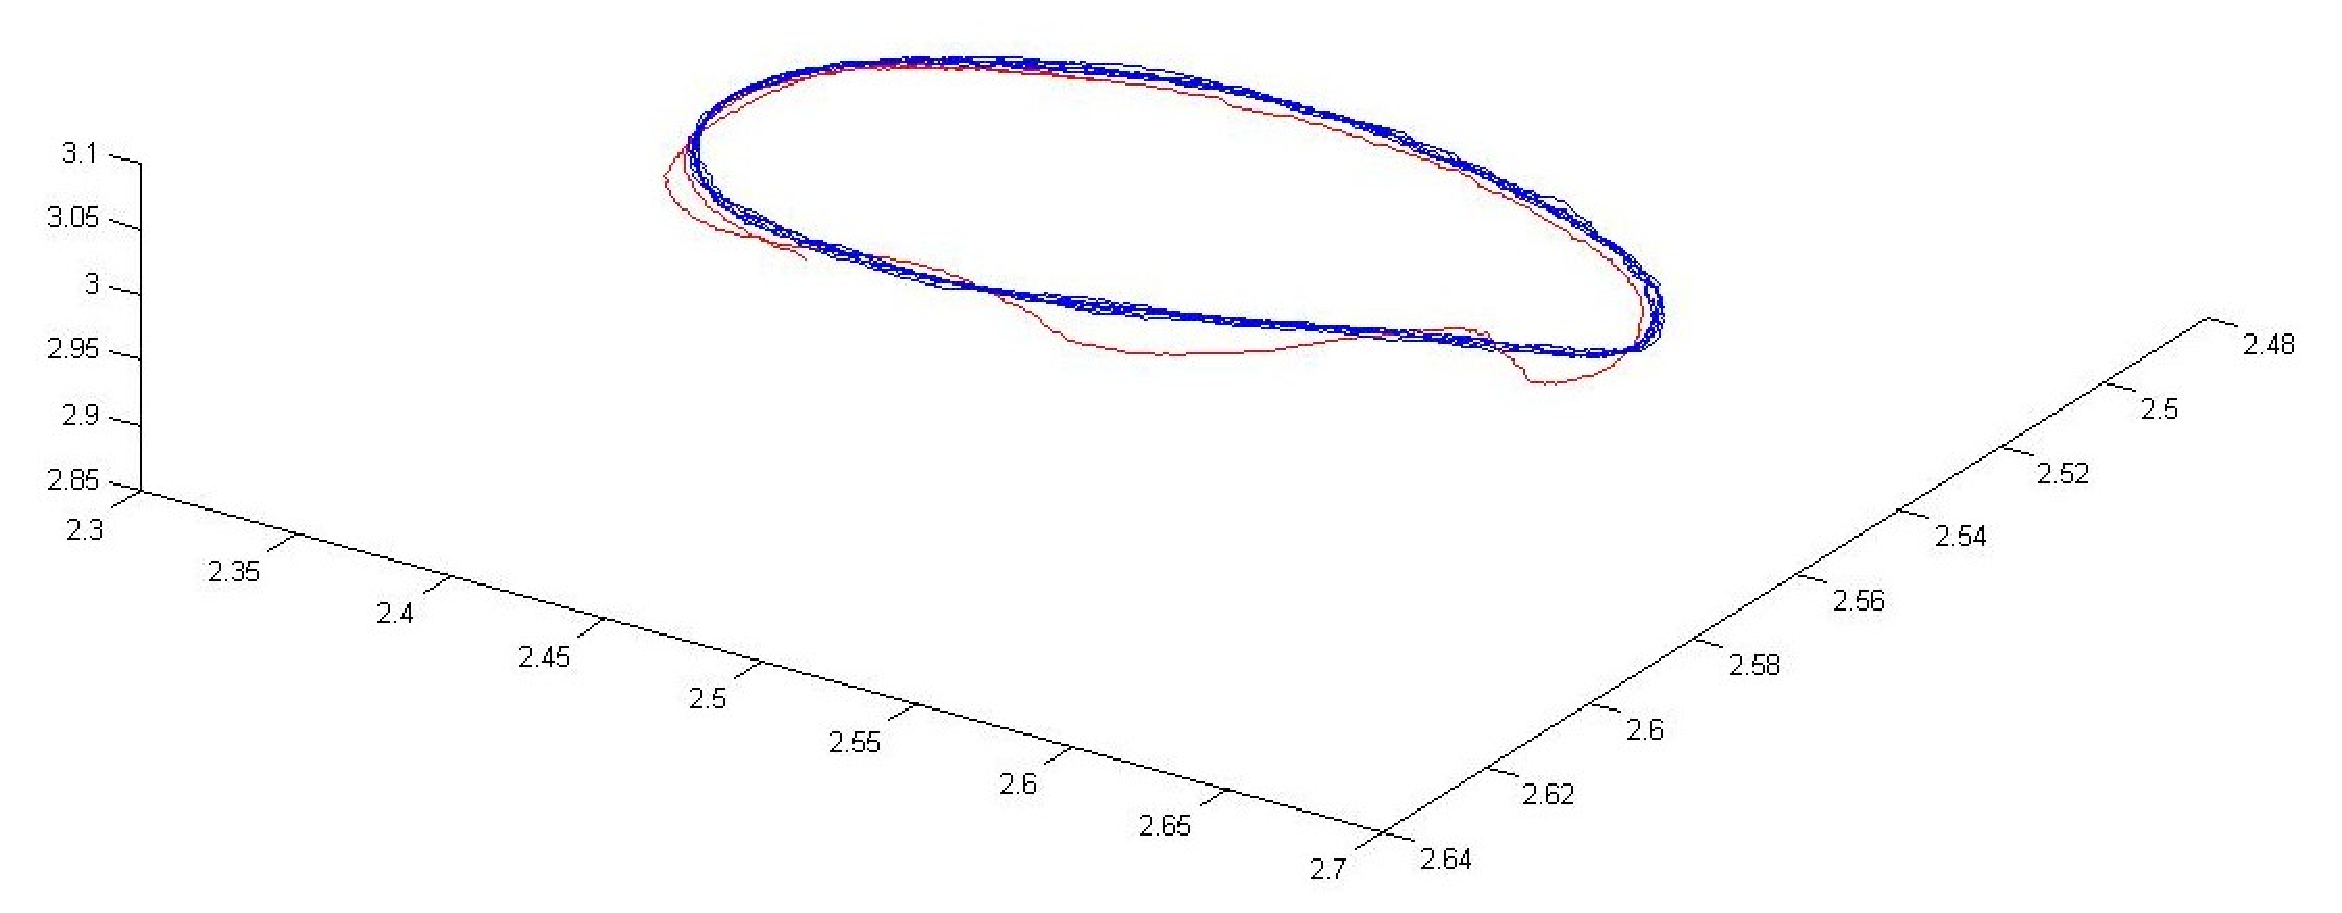
\psfig{file=figures/tam_uniform_field.eps,width=0.8\textwidth}}
  \caption{TAM measurements in a uniform field}
  \label{fig:TAMUniformField}
\end{figure}

Since the gyroscope and accelerometers were determined to be useless for the observer based controller, and the course sun sensors only able to detect motion about the z-axis, the triple-axis magnetometer remained the only sensor onboard that had the capability of detecting the nutation required for the MMS controller.

The baseline path established for TableSat in the absence of nutation (Figure \ref{fig:TAMUniformField}) should be able to be compared to readings during a live run of the system and any offsets used to quantify nutation.  The same process of rotating the TableSat under a constant thrust was repeated four more times.  Each time a 200g brass weight was placed on the TableSat's deck at each principle axis $+x, +y, -x, -y$ causing the TableSat to pivot about 14 degrees out of the spin plane which was about the extent its range for nutation.  The TAM voltages for each run are grouped by color and shown in Figure \ref{fig:TAMNutationVoltages}.  Although the paths intersect and measurements are not 1:1 to the TableSat's orientation, there is at least a separation in paths.  Further study found that while the TAM voltages are duplicated between nutation paths, points that occupy the same space in the TAM measurement have different yaw measurements as measured by the course sun sensor.

\begin{figure}[H]
  \centerline{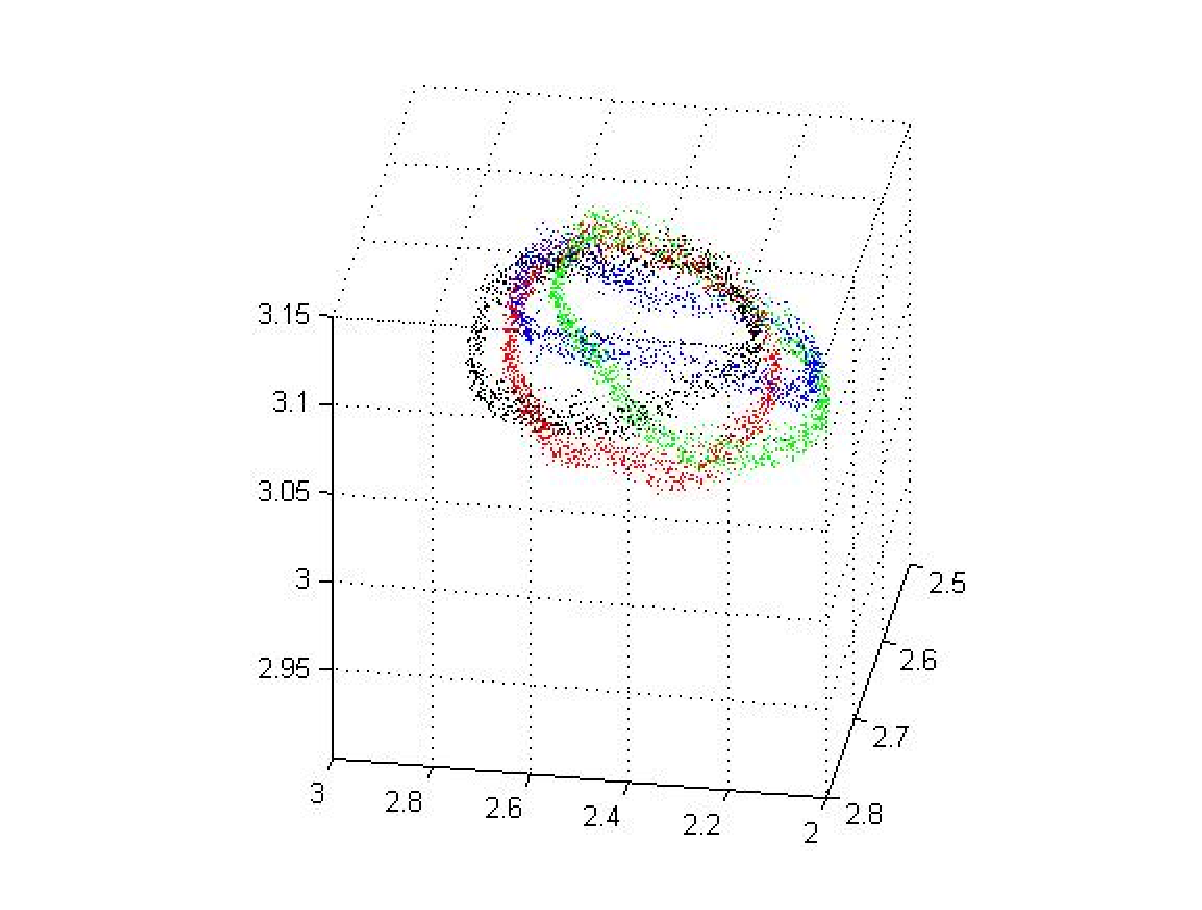
\psfig{file=figures/tam_distinct_tilts_with_good_field.eps,height=4in}}
  \caption{TAM nutation voltages}
  \label{fig:TAMNutationVoltages}
\end{figure}

\section{TableSat State Measurement}
\label{subsec:StateMeasurement}

As covered in the sections above, the only sensors available for state measurement of TableSat 1A for the observer based controller were the course sun sensor and the triple axis magnetometer.  Both of which individually measure a portion of the system's attitude and leave the system's body rate unmeasured.

Combining the measurements of the course sun sensor and triple axis magnetometer provided high confidence in the yaw measurement and rough estimates about the roll and pitch nutations.  An algorithm was developed that started with the course sun sensor and through equation \ref{eqn:CSSResultantForce} produced a measurement of yaw.  The TAM calibration data was synthesized to create a reference table of TAM readings at each of the five paths (steady, and the four nutations shown in Figure \ref{fig:TAMNutationVoltages}).  This reference table along with the equation to determine yaw from the course sun sensor are comined through a method descibed in \ref{subsec:SampleAttitudeCalculation} to approximate the TableSat's attitude.

\begin{table}[H]
  \centering
  \begin{tabular}{c|ccc|ccc}
    \hline
    Yaw   & & Steady & & & $+X \ 14^o$ & \\ \hline
    (deg) & $TAM_x$ (V) & $TAM_y$ (V) & $TAM_x$ (V) & $TAM_x$ (V) & $TAM_y$ (V) & $TAM_x$ (V)  \\ \hline
    0 & $S_{x0}$ & $S_{y0}$ & $S_{z0}$ & $+X_{x0}$ & $+X_{y0}$ & $+X_{z0}$ \\ \hline
    1 & $S_{x1}$ & $S_{y1}$ & $S_{z1}$ & $+X_{x1}$ & $+X_{y1}$ & $+X_{z1}$ \\ \hline
    ... & & & & & &  \\ \hline
    Yaw   & & $+Y \ 14^o$ & & & $-X \ 14^o$ & \\ \hline
    (deg) & $TAM_x$ (V) & $TAM_y$ (V) & $TAM_x$ (V) & $TAM_x$ (V) & $TAM_y$ (V) & $TAM_x$ (V)  \\ \hline
    0 & $+Y_{x0}$ & $+Y_{y0}$ & $+Y_{z0}$ & $-X_{x0}$ & $-X_{y0}$ & $-X_{z0}$ \\ \hline
    1 & $+Y_{x1}$ & $+Y_{y1}$ & $+Y_{z1}$ & $-X_{x1}$ & $-X_{y1}$ & $-X_{z1}$ \\ \hline
    ... & & & & & &  \\ \hline
    Yaw   & & $-Y \ 14^o$ & &  \\ \hline
    (deg) & $TAM_x$ (V) & $TAM_y$ (V) & $TAM_x$ (V)  \\ \hline
    0 & $-Y_{x0}$ & $-Y_{y0}$ & $-Y_{z0}$  \\ \hline
    1 & $-Y_{x1}$ & $-Y_{y1}$ & $-Y_{z1}$  \\ \hline
    ... & & & & & &  \\ \hline
  \end{tabular}
  \caption{TAM calibration reference table}
  \label{tbl:TAMCalibration}
\end{table}

\subsection{Sample Attitude Calculation}
\label{subsec:SampleAttitudeCalculation}

This example will go through a sample calculation of the nutation based on a single set of course sun sensor and triple axis magnetometer voltage measurements.

\subsubsection{Scan Sensor Voltages}

The base station submits message id 20 to TableSat which responds with a message 63 with a payload containing 15 floats (timestamp, 6 photodiodes, 4 accelerometrs, gyroscope, and 3 triple-axis magnetometer).

\subsubsection{Calculate Yaw From Course Sun Sensor}

Using sample CSS voltages from the photodiodes of 0.37247, 0.30899, 1.18370, 2.40020, 1.80500, and 0.44052.  The TSatPy python package whose development is detailed in Chapter \ref{chap:TSatPy} uses equation \ref{eqn:CSSResultantForce} to convert the sensor voltages into a meaningful state.

\begin{singlespace}
  \begin{minted}[mathescape,
               linenos,
               numbersep=10pt,
               frame=lines,
               framesep=2mm]{python}
import TSatPy
import numpy as np

css_v = [0.37247, 0.30899, 1.18370, 2.40020, 1.80500, 0.44052]

pda = TSatPy.Sensor.PhotoDiodeArray()
pda.update_state(css_v)
vector, radians = pda.x.q.to_rotation()

print "A %g radian (%d degree) rotation about <%g, %g, %g>" % (
    radians, radians / np.pi * 180,
    vector[0,0], vector[1,0], vector[2,0])

# Prints out
# A 3.34585 radian (191 degree) rotation about <-0, -0, -1>
  \end{minted}
  \nocite{minted}
\end{singlespace}

\subsubsection{Calculate TAM Nutation Reference Data}

Figure \ref{fig:TAMNutationVoltages} shows that while the TAM readings vary enough to be noticeable for large nutations the signal contain a fair quantity of noise.  In order to use the triple-axis magnetometer to quantify nutation for the observer based controller, the data in Table \ref{tbl:TAMCalibration} needs to be summarized to five data points for a yaw angle of 191 degrees.  When running the estimator, TAM sensor values can be compared to the five reference nutation points of flat, +x down, +y down, -x down, and -y down.

The method chosen for creating the five reference points starts with collecting about 2400 data points with corresponding TAM and course sun sensor voltages.  The voltages for each nutation setting were grouped into 1 degree increments.  Multiple rotations created some overlap in each degree measurements.  The final reference value for each degree was calculated through a weighted average of a specified smoothing window.

Figure \ref{fig:TAMNutationReference} shows the result of the nutation reference values for 5, 15 and 25 degree smoothing windows.  At $\pm 15$ degrees, an adequate level of noise was filtered out without causing over smoothing.  At this level, each of the 191 degree reference values would be a weighted average of about 200 of the original calibration points.

\begin{figure}[H]
  \begin{subfigure}[h!]{0.5\textwidth}
    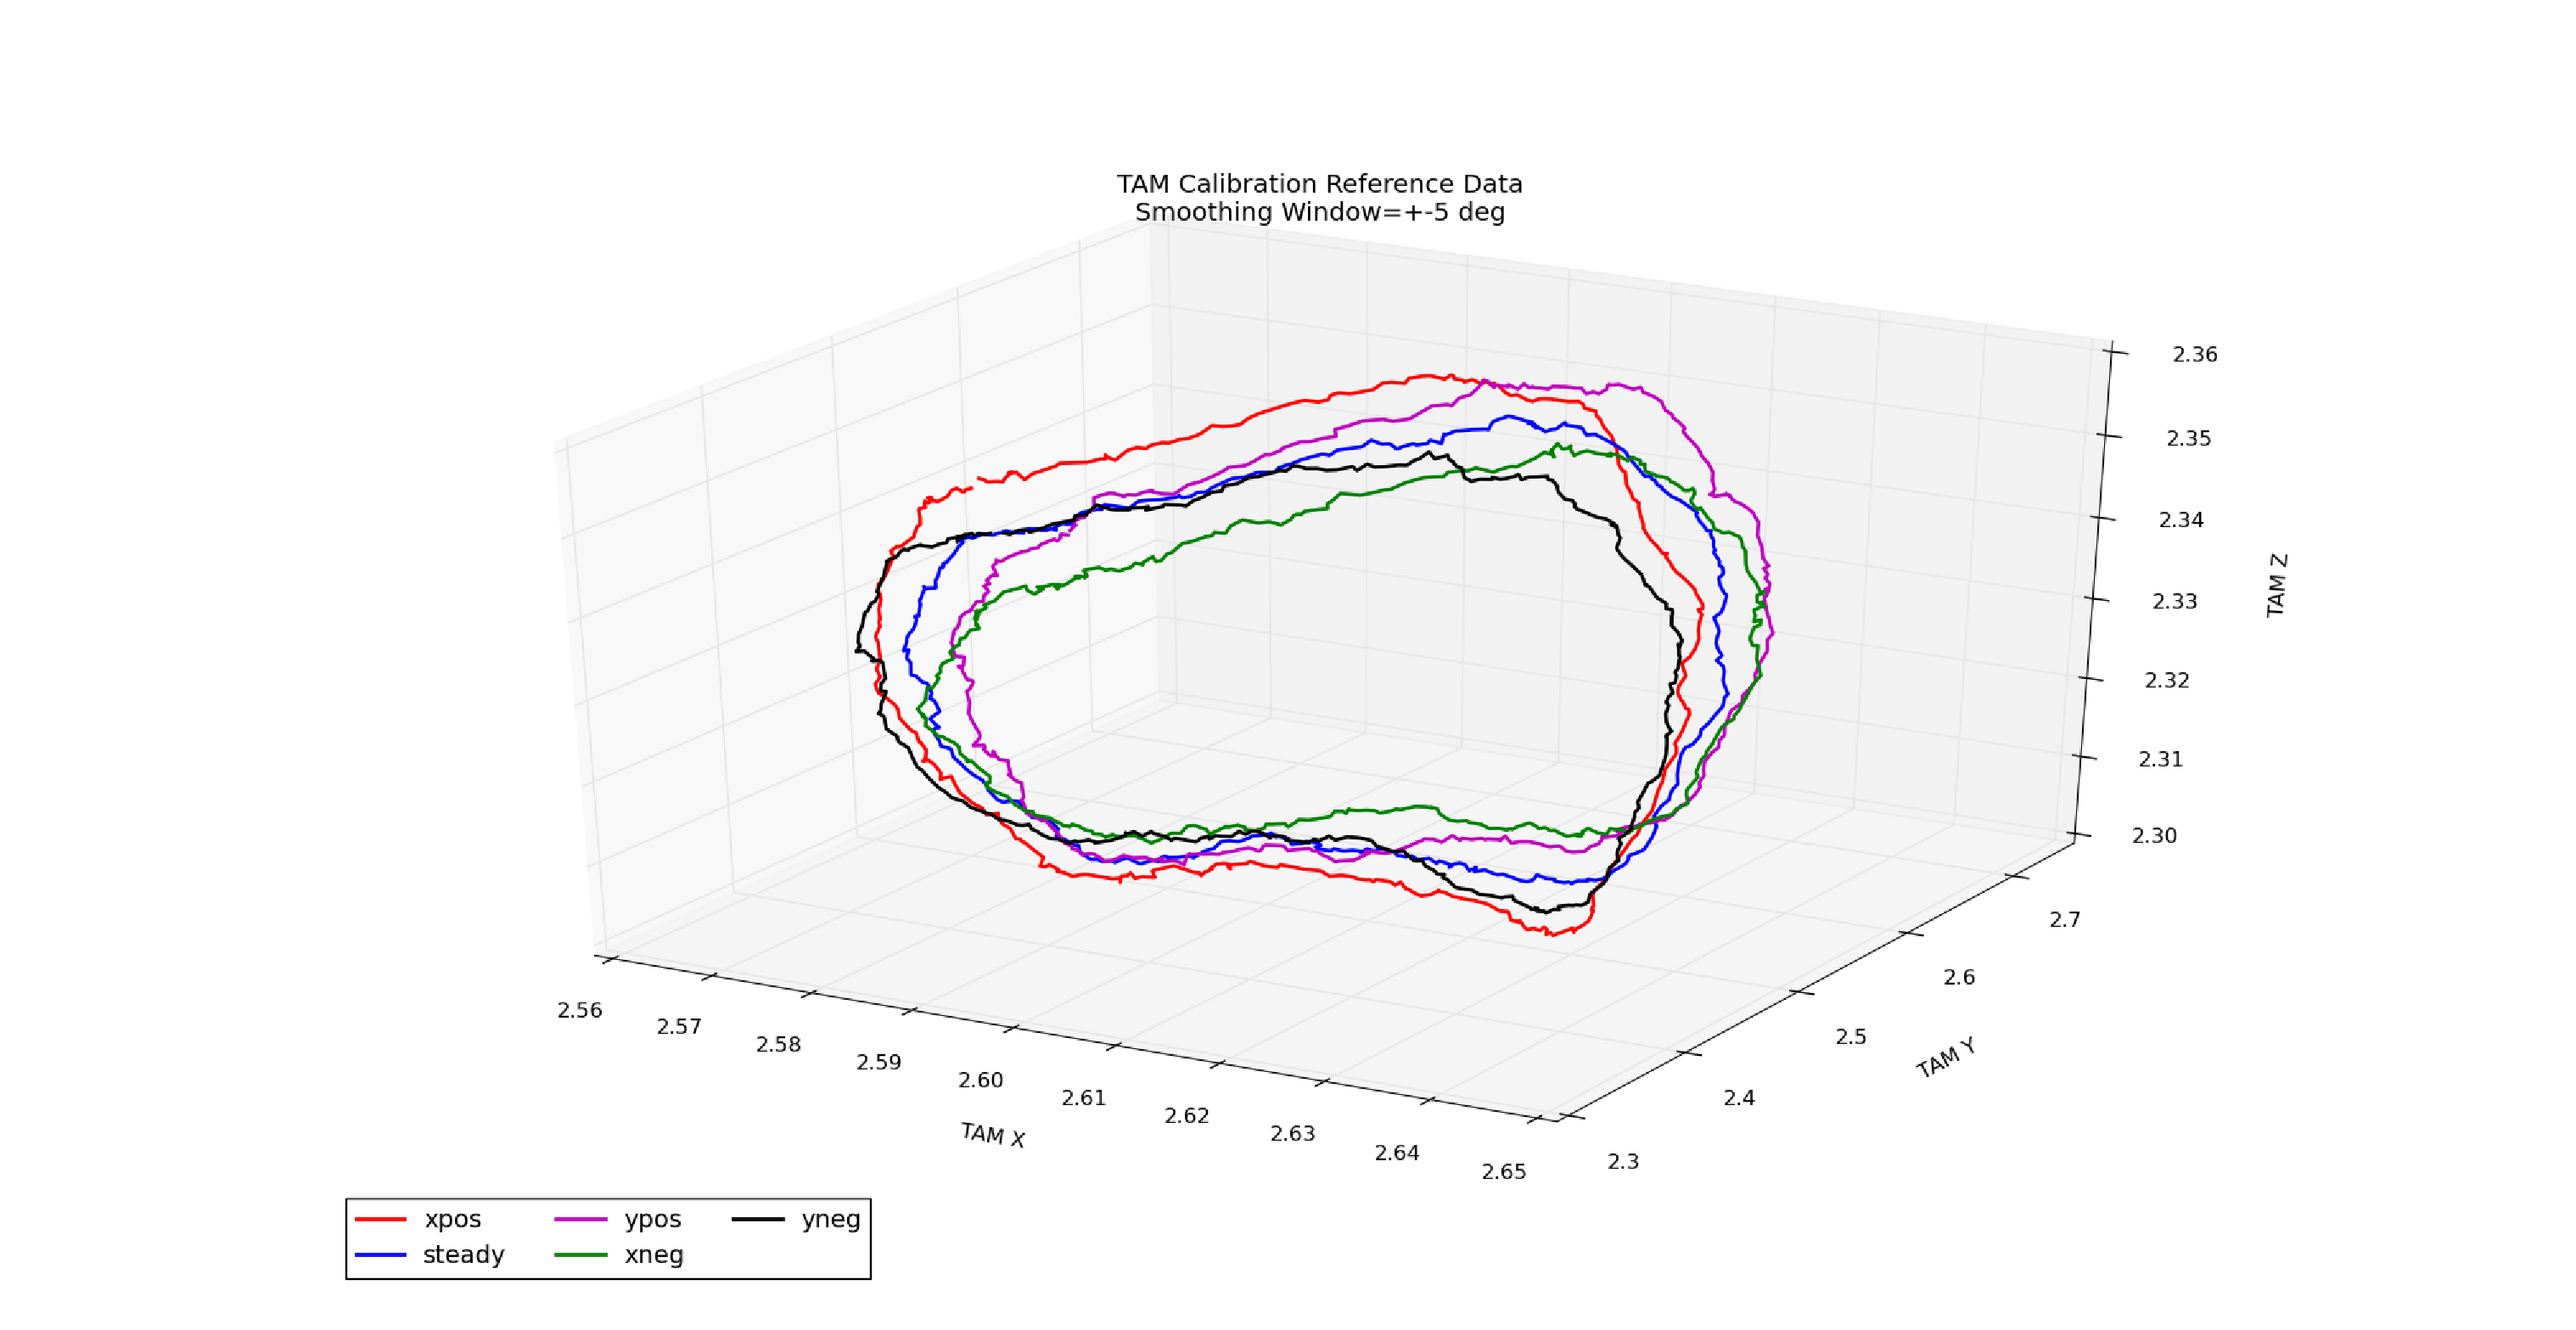
\includegraphics[width=\textwidth]{figures/tam_calibration_ref_5deg_smoothing.eps}
    \caption{$\pm 5^o$ smoothing}
    \label{fig:TAM5degCalibration}
  \end{subfigure}
  ~
  \begin{subfigure}[h!]{0.5\textwidth}
    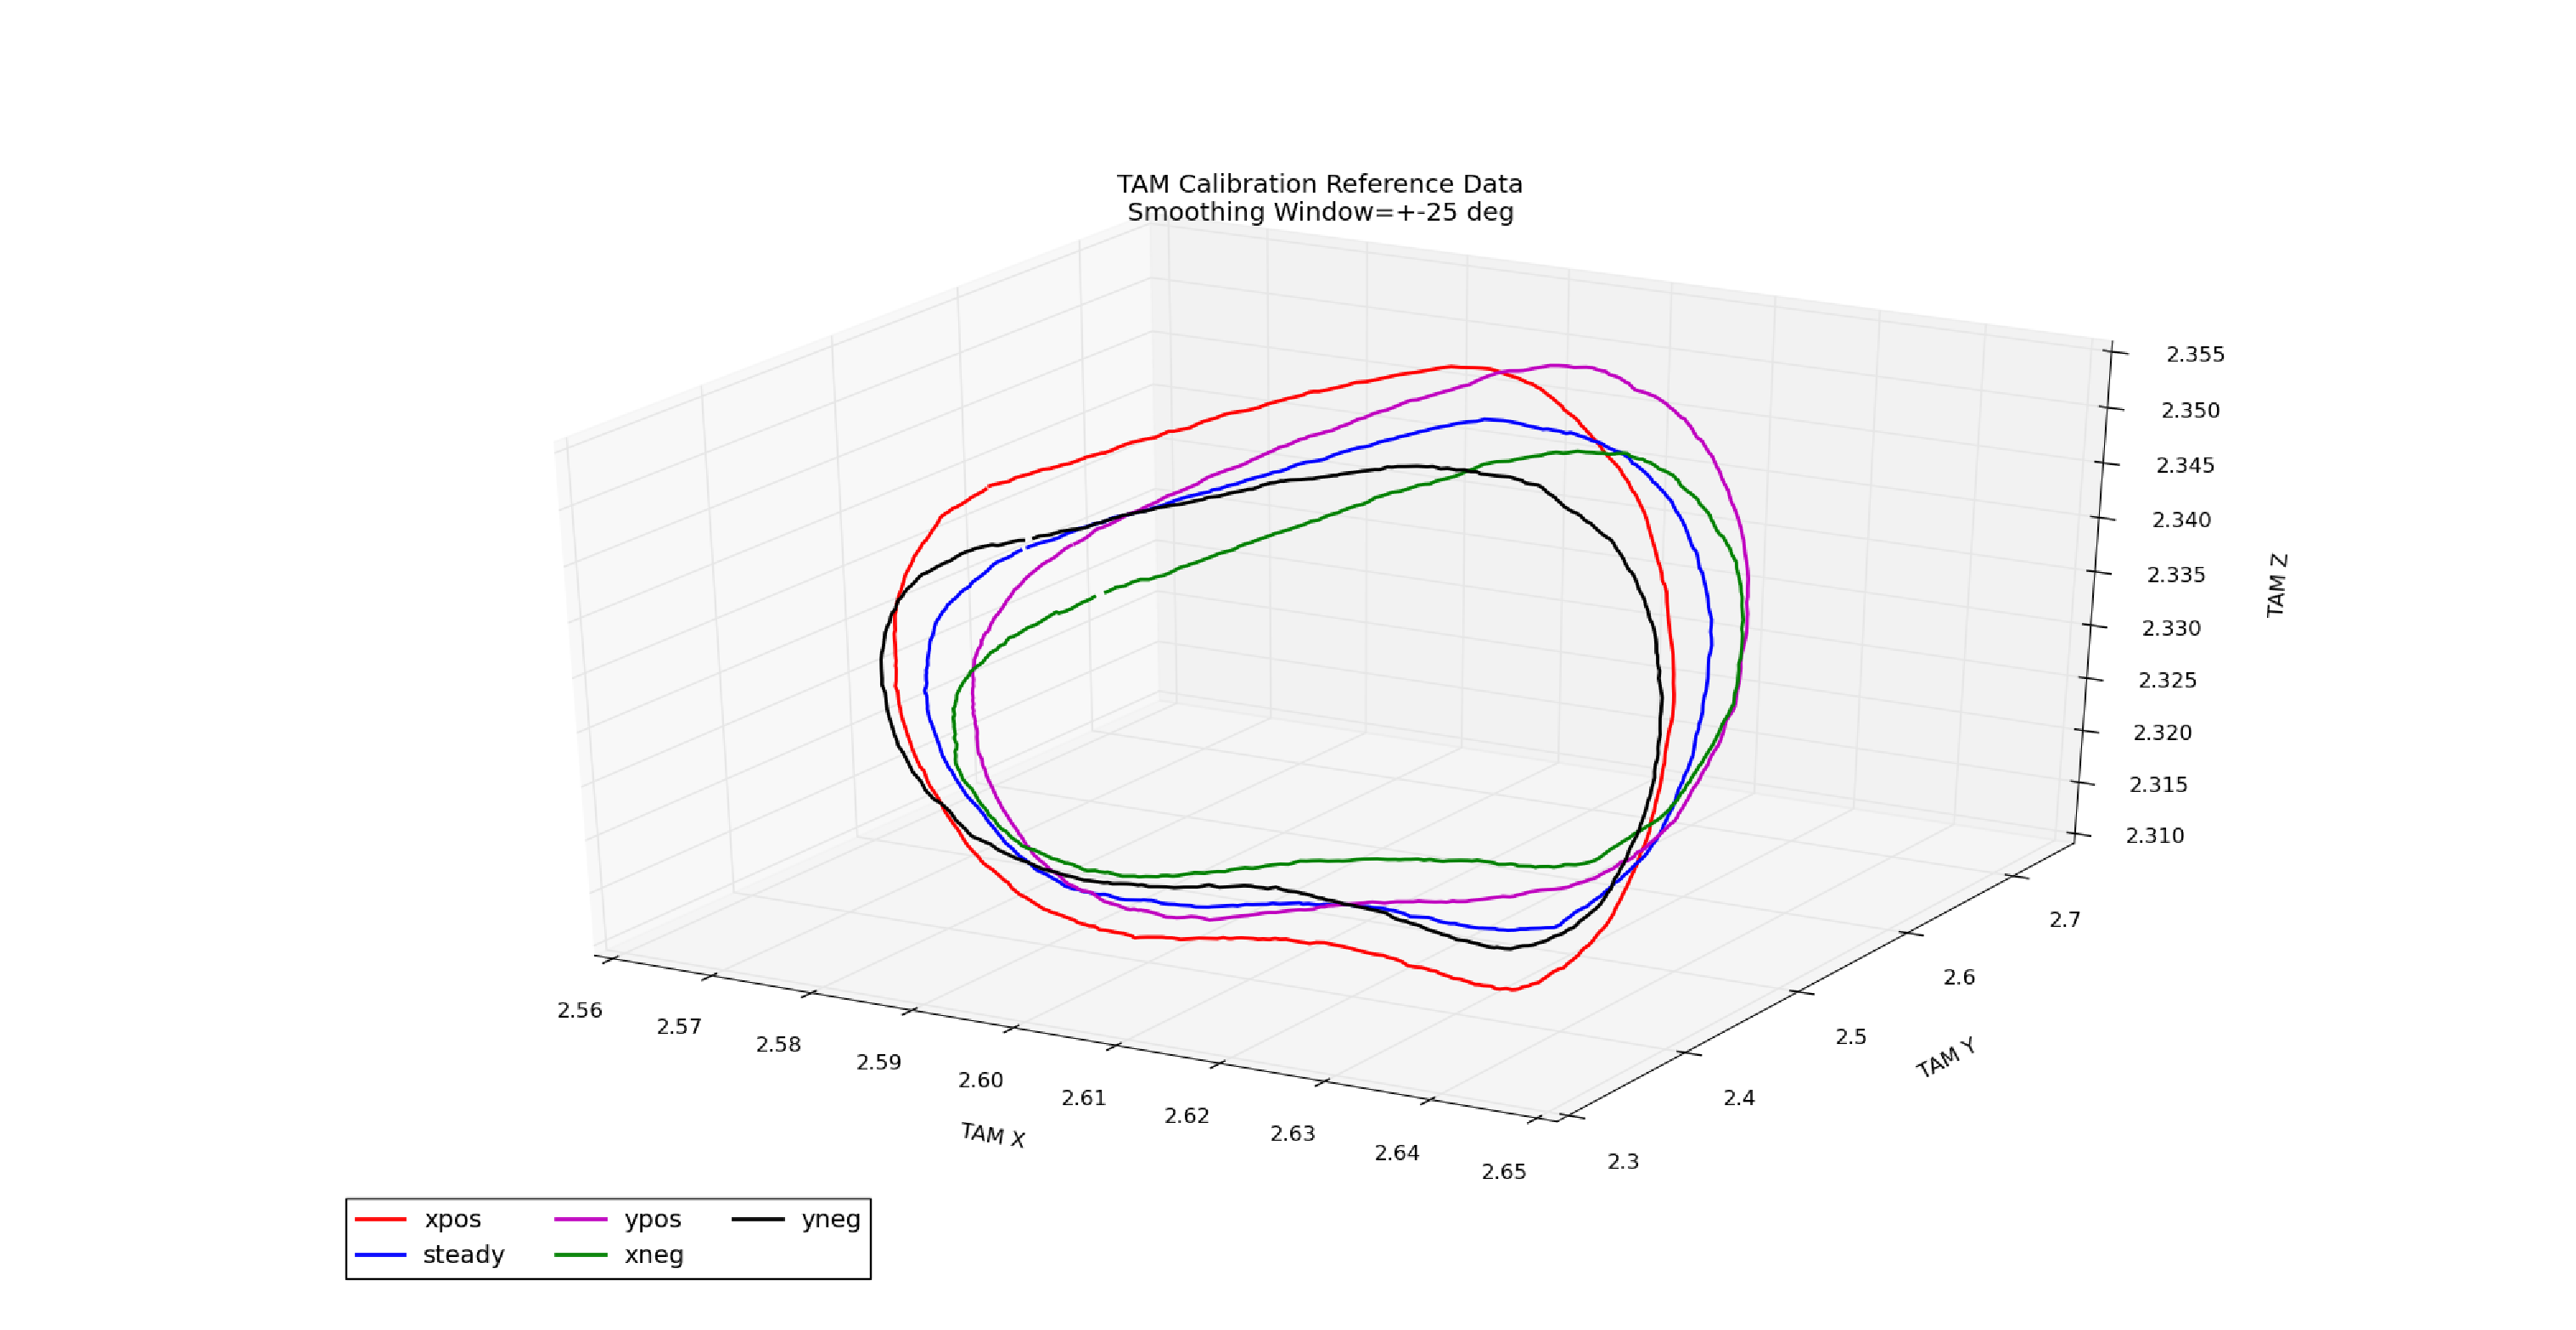
\includegraphics[width=\textwidth]{figures/tam_calibration_ref_25deg_smoothing.eps}
    \caption{$\pm 25^o$ smoothing}
    \label{fig:TAM25degCalibration}
  \end{subfigure}

  \begin{subfigure}[h!]{0.8\textwidth}
    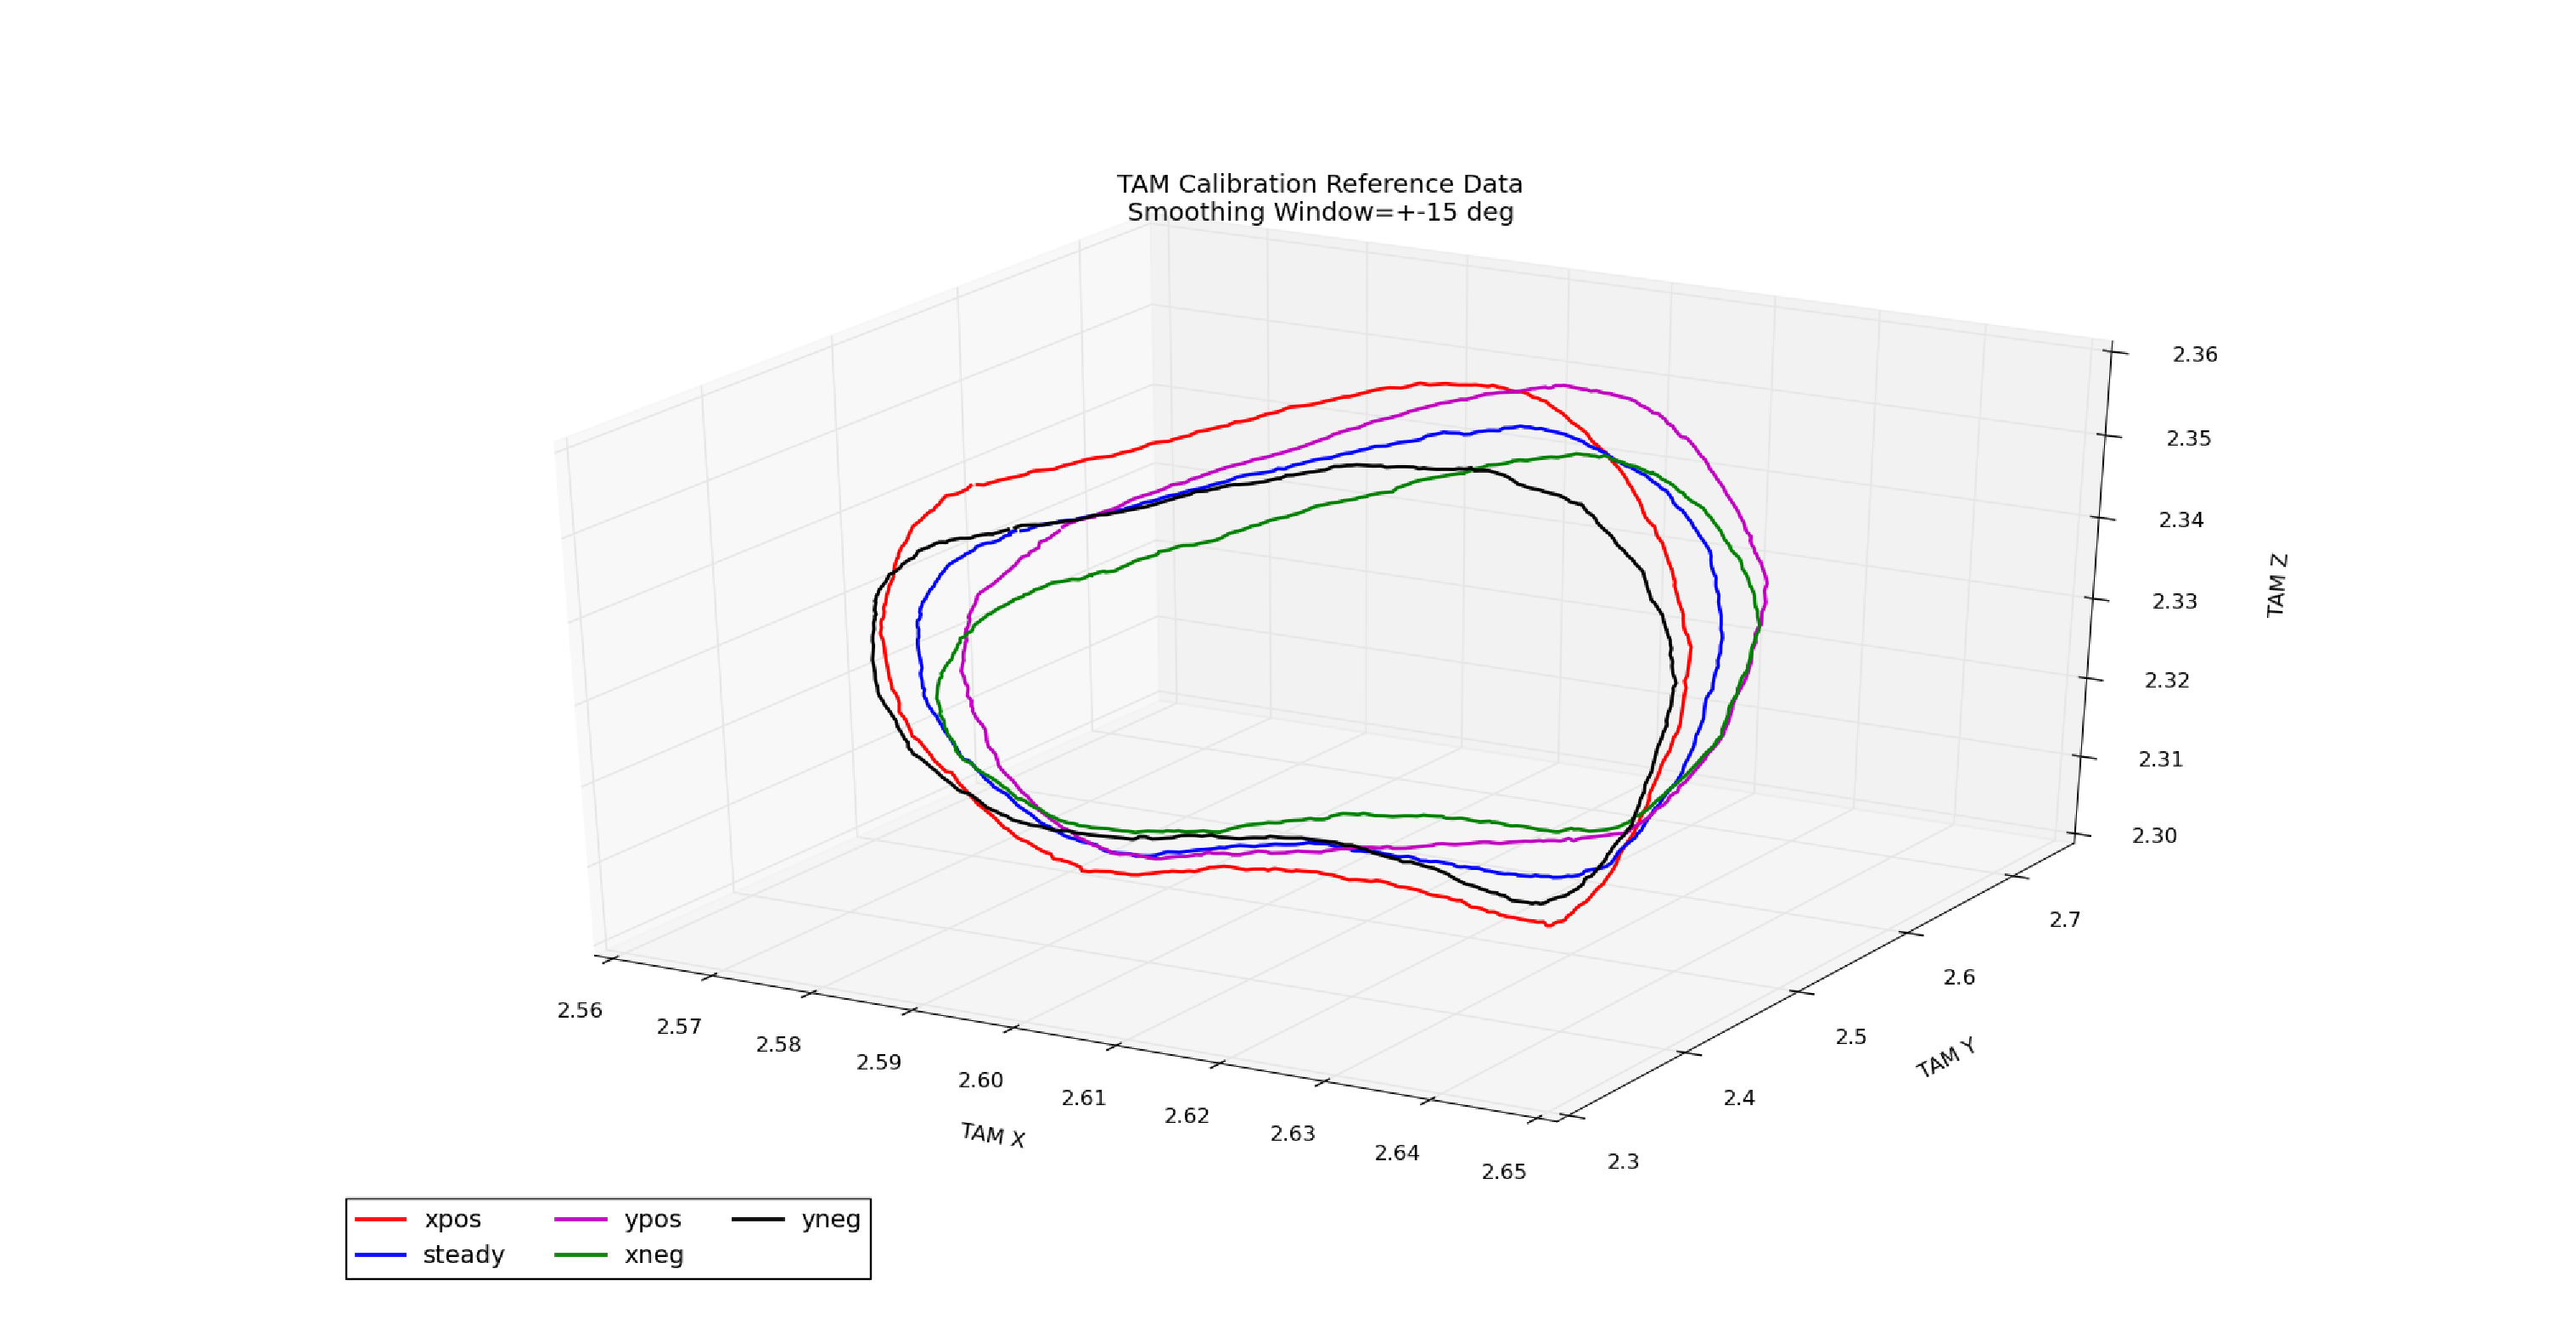
\includegraphics[width=\textwidth]{figures/tam_calibration_ref_15deg_smoothing.eps}
    \caption{$\pm 15^o$ smoothing}
    \label{fig:TAM15degCalibration}
  \end{subfigure}
  \caption{TAM Nutation Reference Values}
  \label{fig:TAMNutationReference}
\end{figure}

The cross shown in Figure \ref{fig:TAMRef191} illustrates the difference in the four nutation reference points compared to the stable point for a 191 degree yaw.  Figure \ref{fig:TAMPoints191} shows just how much noise is smoothed out by the calibration process as the original data points are plotted against the reference nutation voltages.

\begin{figure}[H]
  \centerline{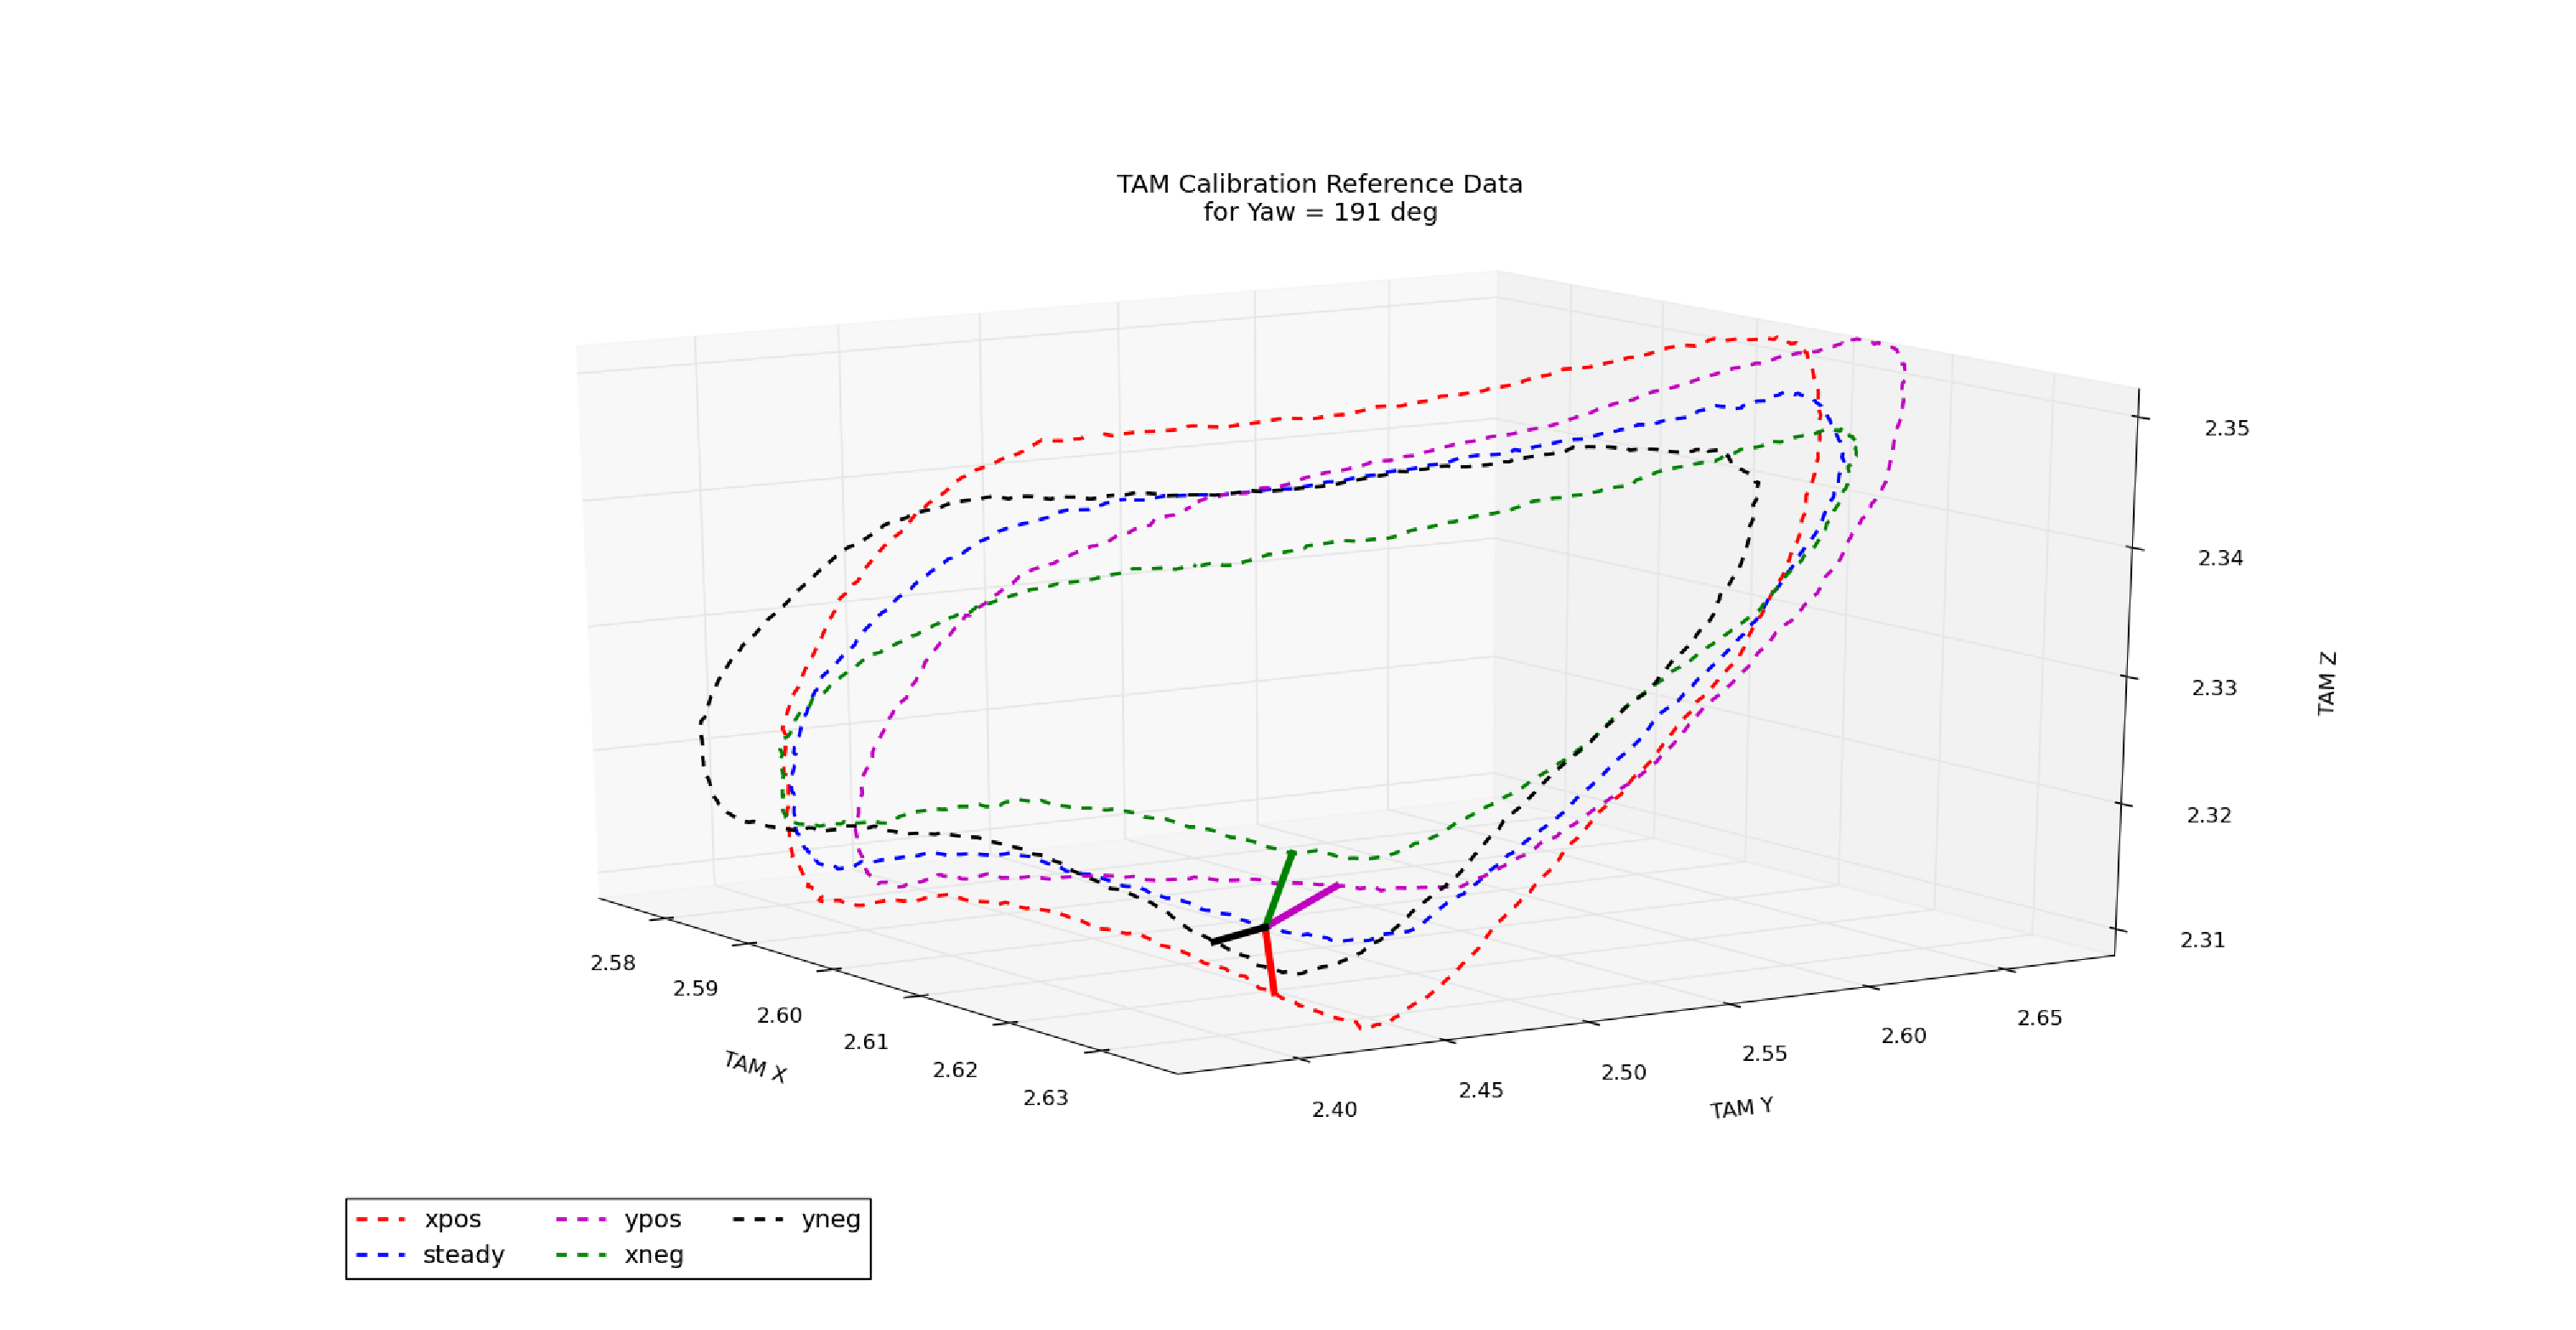
\psfig{file=figures/tam_calibration_ref_for_yaw_191.eps,height=3in}}
  \caption{TAM reference voltages for 191 degree yaw}
  \label{fig:TAMRef191}
\end{figure}

\begin{figure}[H]
  \centerline{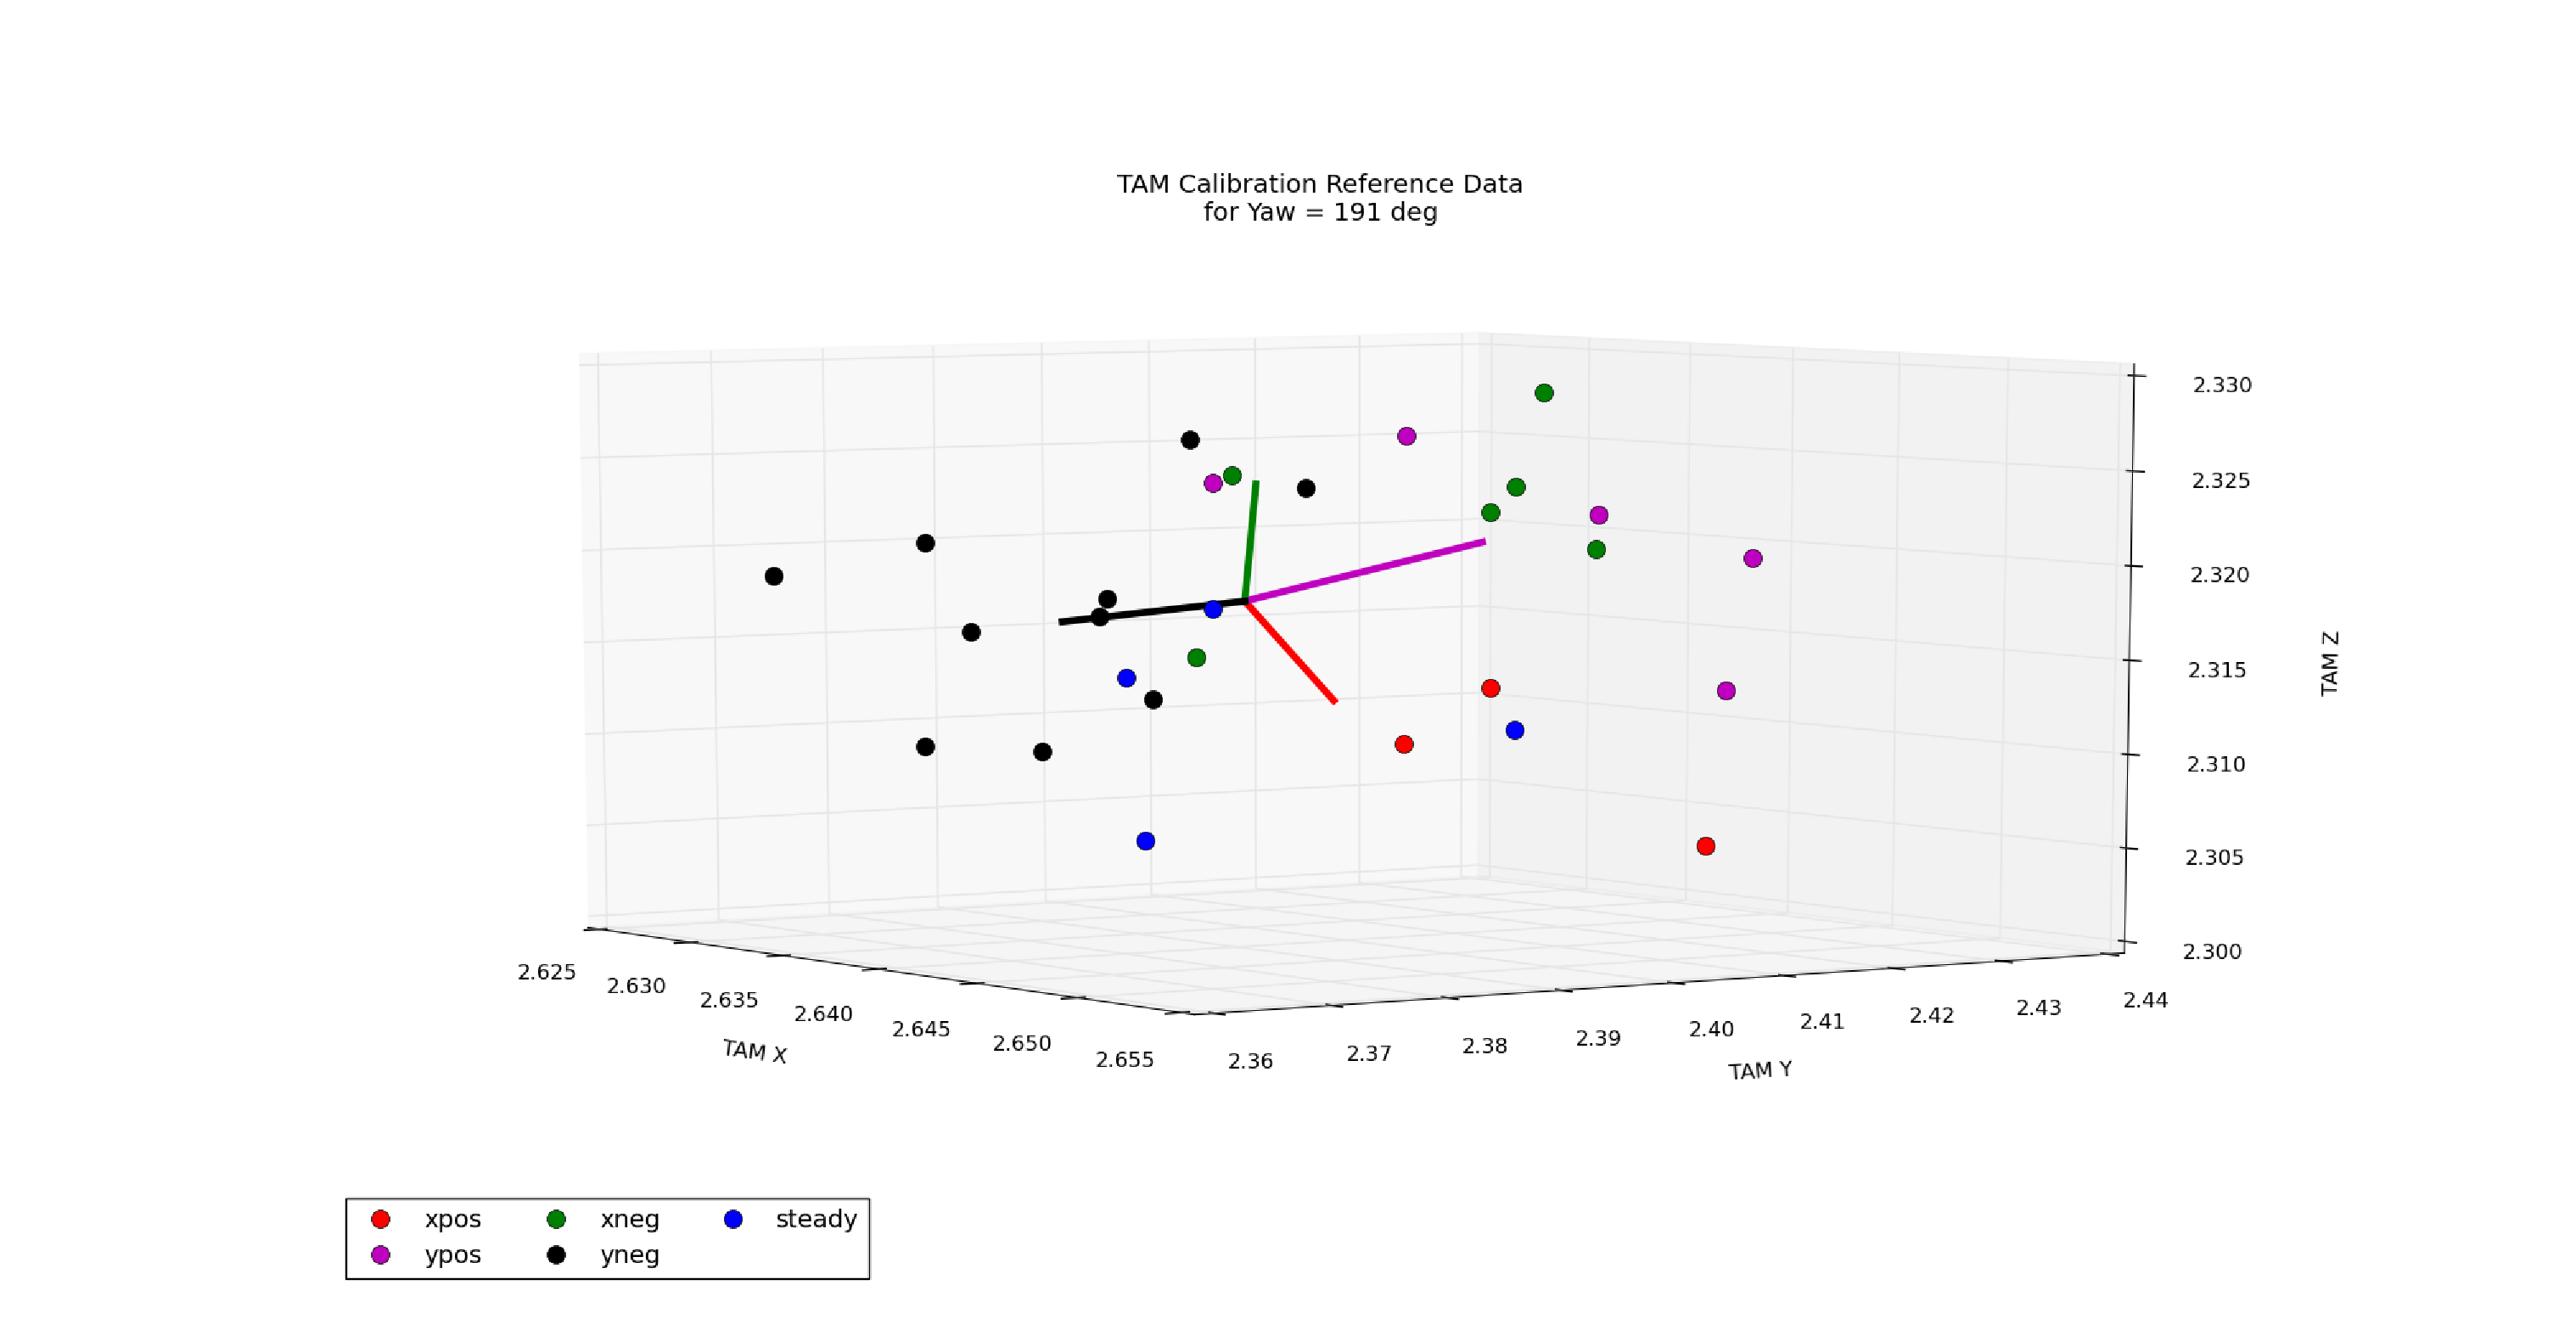
\psfig{file=figures/tam_calibration_191_degree_pts.eps,height=3in}}
  \caption{TAM reference voltages for 191 degree yaw}
  \label{fig:TAMPoints191}
\end{figure}

\subsubsection{Estimating the Nutation}

Taking one of the points from yneg calibration data to complete the example, Table \ref{tbl:TAMSamplePoints} lists the test point along with the reference values obtained from the calibration algorithm above.  The test point, plotted it Figure \ref{fig:TAMPoint191} is nearest to the reference yneg value, but there is a large gap between the measured value and it associated reference, and other test points as in \ref{fig:TAMPoints191} are far closer to another reference point than its own.

\begin{table}[H]
  \centering
  \begin{tabular}{lc}
    \hline
    Test Point       & $(2.63, 2.37, 2.32)$ \\ \hline
    Steady Reference & $(2.63, 2.40, 2.32)$ \\ \hline
    xpos Reference   & $(2.63, 2.42, 2.31)$ \\ \hline
    ypos Reference   & $(2.64, 2.42, 2.32)$ \\ \hline
    xneg Reference   & $(2.64, 2.39, 2.32)$ \\ \hline
    yneg Reference   & $(2.63, 2.39, 2.32)$ \\ \hline
  \end{tabular}
  \caption{TAM sample reference points}
  \label{tbl:TAMSamplePoints}
\end{table}


\begin{figure}[H]
  \centerline{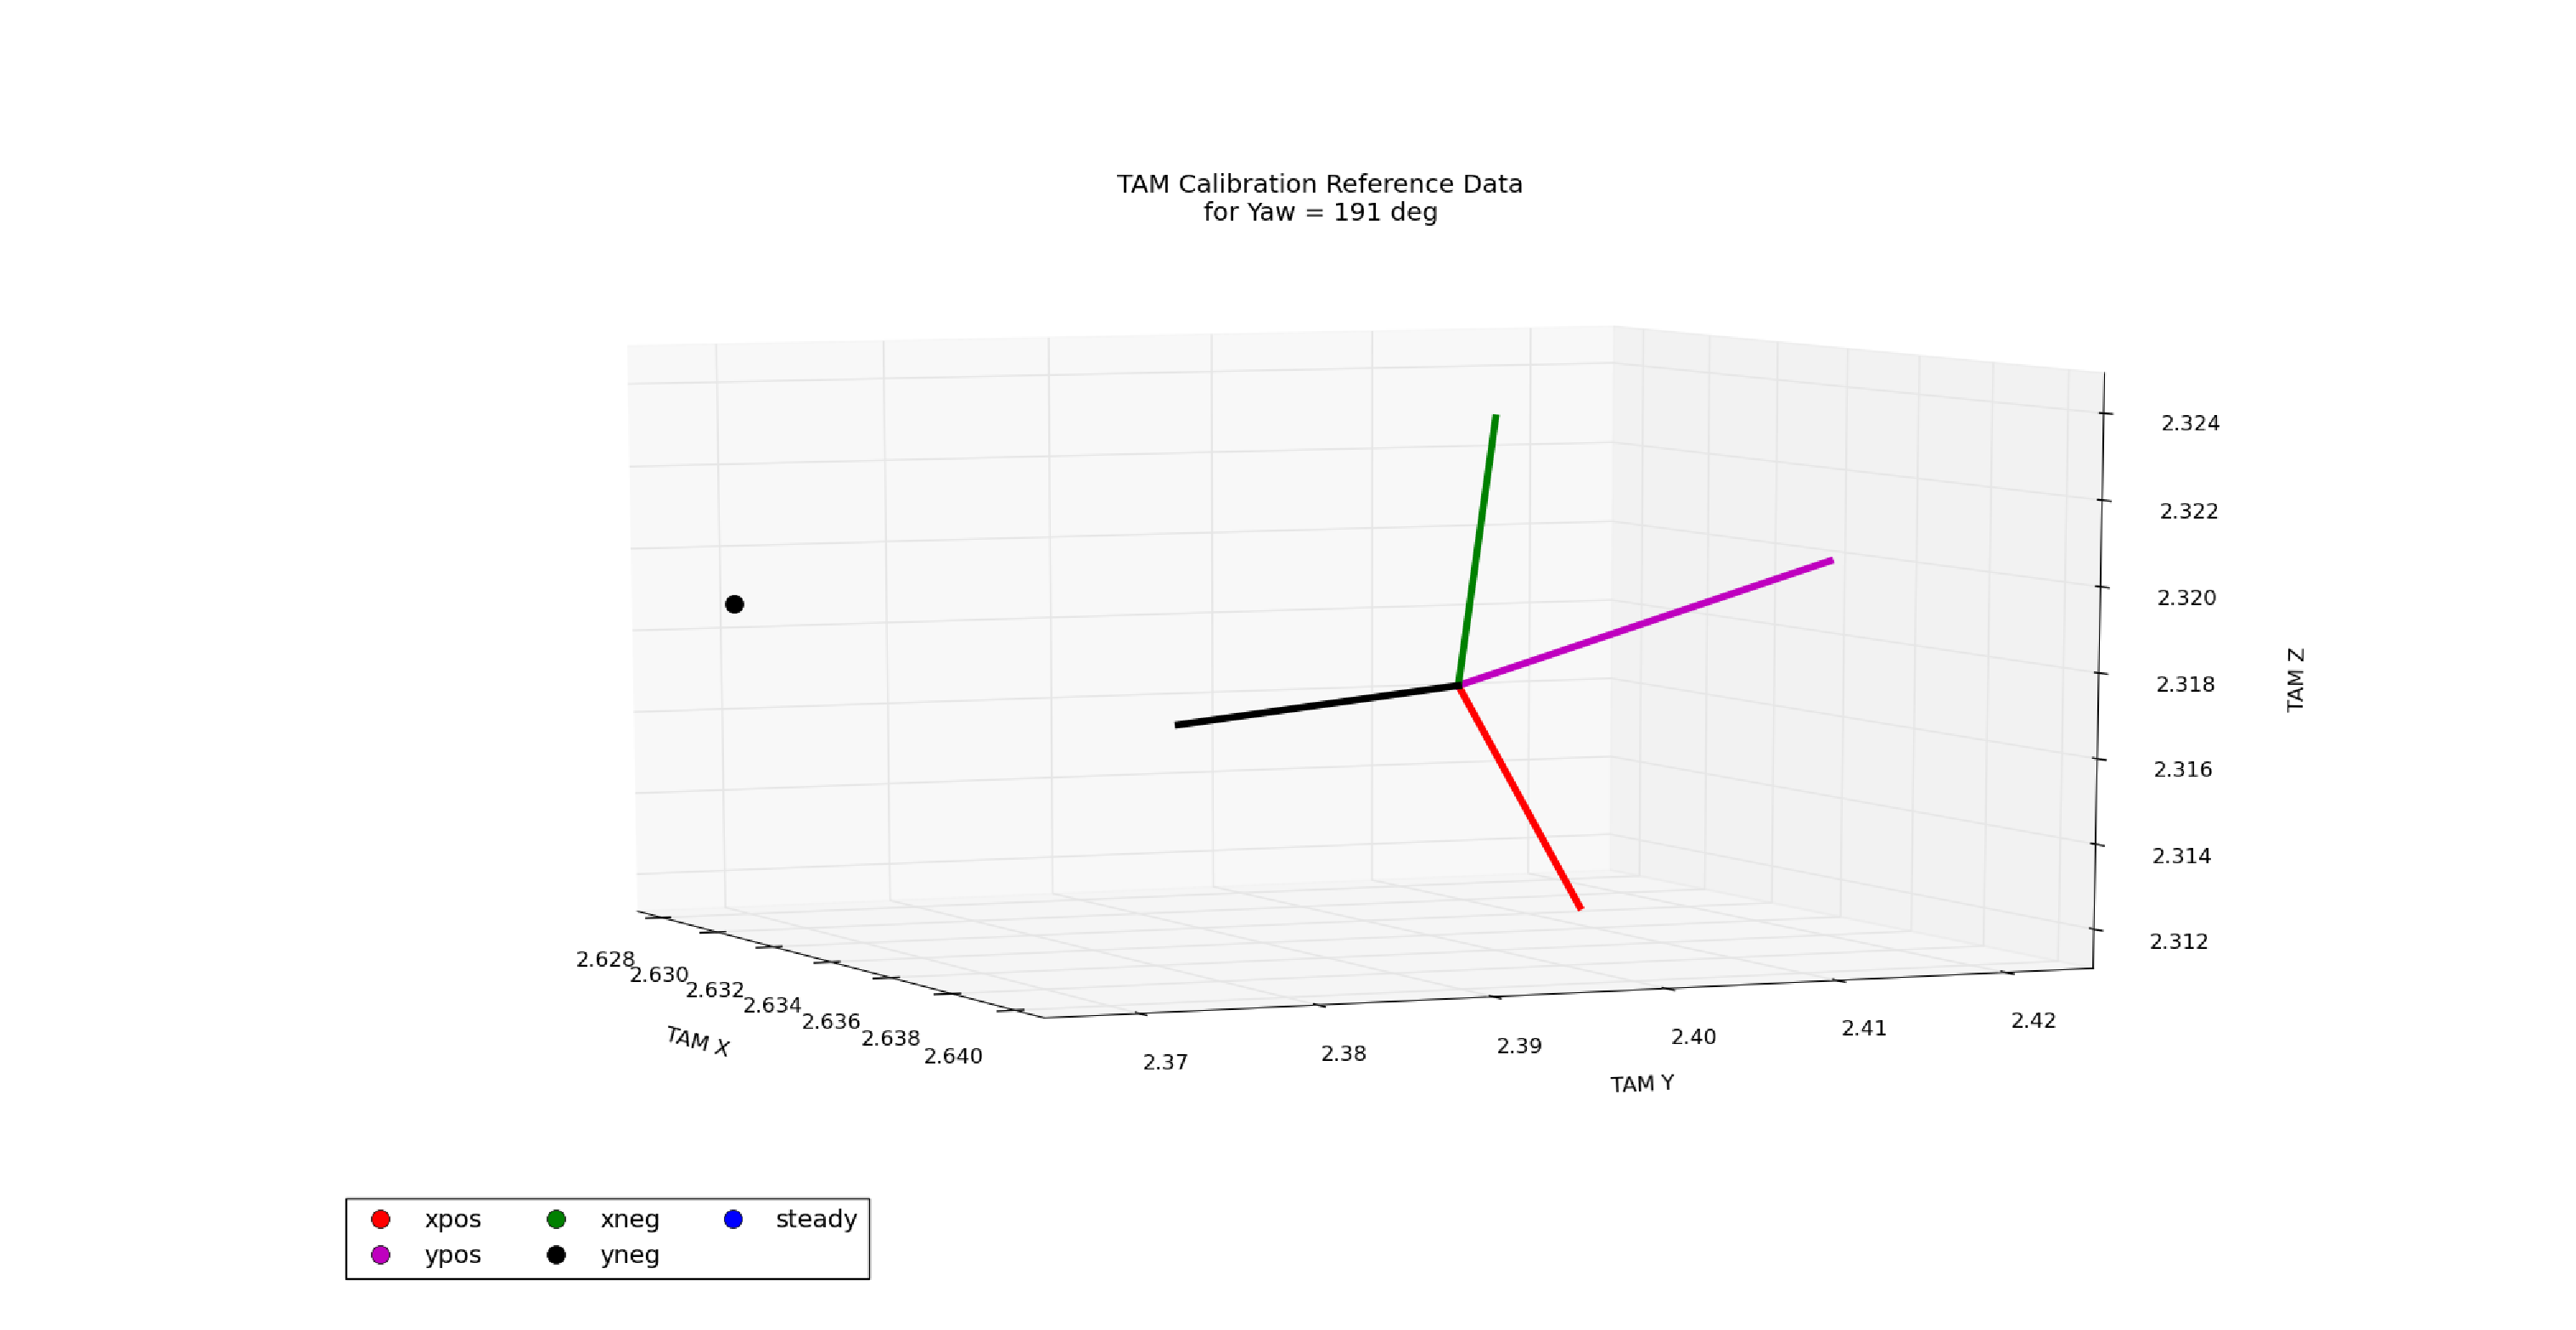
\psfig{file=figures/tam_calibration_191_degree_pt.eps,height=3in}}
  \caption{TAM sample data point for nutation calculation}
  \label{fig:TAMPoint191}
\end{figure}

In order to determine the best approximation for the measured nutations a number of combinations of approaches were attempted including using the proportion between two estimates, normalizing the reference vectors, projecting the point to the plane consisting of the two nearest vectors, and creating a conversion of the x and y vectors to an orthogonal space.  Some cases provided slightly lower classification error rates when run against the original calibration test set, but any improvements were not significant.  For simplicity and speed, the measurement estimate for nutation was reduced to a nearest neighbor classification \cite{nearestneighbor} where the closest reference point won out.

Despite the improved speed and simplicity, this classification method has some large faults.  The biggest of which is the jitter that will be fed into the estimator since with no continuum of values, the nutation state will jump between the five calibration states of flat, and $14^o$ nutations.  Further work should be focused on refining this technique.

\section{Messages Between TableSat and the Base Station}


\subsection{Message Protocol}
\label{subsec:UDPTCP}

Communication between the controller and the experimental TableSat is negotiated over a User Datagram Protocol (UDP) socket.  Both the controller and TableSat read and write over port 9877.  UDP is used for a stateless connection more generally used for pushing data over a large number of connections.  The other common communication protocol is Transmission Control Protocol (TCP) where a session is established between server and client and successful transferral of data is acknowledged by the recipient.

Advantages and disadvantages exist between the TCP and UDP protocols and became a critical factor in influencing the design of TableSat 1A base station controller. Section \ref{sec:Simulink} goes into further detail in how this difference in protocols cropped up early in the development of the base station controller where the combination of Matlab Simulink with a UDP communication protocol produced a very fragile system.

A UDP message transmission is done in a ``fire and forget'' fashion.  The message header can generally include the originating hosts ip address and port so that the server knows where to send the response.  The session-less nature of UDP means that the originating server sends the message, but does not receive confirmation that the message transmitted successfully as with TCP where ever interaction is followed up with an acknowledgment from the other host.

The advantage to using UDP for the UNH TableSat 1 is that the satellite side code could be largely based off of Melissa Vess' work on her TableSat thesis where the control loop was implemented on-board, and the UDP connection was used to infrequently poll for data or modify sensor calibration values.  The UDP connection has the slight advantage of being able to transmit and receive packets without needing to wait for acknowledgments.  This could save a small fraction of time, but on modern hardware and with the small bandwidth usage this advantage is negligible.

Disadvantages to a UDP implementing the control interface through UDP include the possibility of packet loss where the sender submits a packet, but it gets corrupted or dropped.  Since UDP is a stateless connection, the sender doesn't wait for an acknowledgment which in this case would not come. This issue is handled by the communications module.  If the control loop rate on both updating the actuator voltages and polling sensor data is fast enough, a dropped packet would not matter much since a new updated set of values would be soon to follow.  Issues could be caused if the completion of a code loop was dependent on a packet coming in.  If dropped, the control loop could block until the next packet is received.  This was one issue encountered in the project version [sec:ControlLoopinSimulink].


\subsection{Message Definitions}
\label{subsec:MessageDefinitions}


The packet structure used for this project is the same as used by Melissa Vess \cite{vessthesis}. Each UDP packet is comprised of a packet header and data payload.  The packet header format remains constant for all messages containing five octets of data.

\begin{table}[H]
  \centering
  \begin{tabular}{| l | l |}
    \hline
    Header Octet & Description \\ \hline
    h1 & Message Number (0 to 255) \\ \hline
    h2 & Flags (0 - 255) \\ \hline
    h3 & Message Size (0 - 255) \\ \hline
    h4 & Message Size (0 - 255) \\ \hline
    h5 & 0 \\ \hline
  \end{tabular}
  \caption{UDP message headers}
  \label{tbl:UDPMessageHeaders}
\end{table}

The first octet (h1) contains the message number that matches to a predefined list of messages known by both the sender and recipient.  This is used to specify how the data in the payload is to be used.

The second octet (h2) is reserved for flags.  For some messages, flags can be set for additional data.  These are not used in the final implementation of UNH TableSat 1A.

The third (h3) and fourth (h4) header octets define the size of the data's payload, so when reading data in from a buffer, the header can inform the recipient how many bytes need to get read in from the buffer in order to get to the end of the packet.  For payloads less than 256 bytes only the fourth header byte is needed.  For payloads larger than 255 bytes the following formula is used to specify the message size headers.

\begin{subequations}
  \begin{align}
    h4 &= mod(size, 256) \\
    h3 &= floor(size / 256)
  \end{align}
  \label{eqn:UDPSizeHeader}
\end{subequations}

The only meta data provided along with the payload beyond the data's size is an 8 bit message number.  Both UNH TableSat 1A and the control station have identical message list definitions.

\begin{table}[H]
  \centering
  \begin{tabular}{|l|l|l|l|}
    \hline
    Message Id & Payload Size & Data Type & Message Description \\ \hline
    2 & 1 octet & unsigned int & Set run mode \\ \hline
    4 & 1 octet & unsigned int & Set run mode \\ \hline
    18 & 4 x (8 octets) & float & Set fan voltages \\ \hline
    19 & 1 octet & unsigned int & Set log record mode \\ \hline
    20 & 1 octet & unsigned int & Request sensor reading \\ \hline
    22 & 1 octet & unsigned int & End of sensor log \\ \hline
    23 & 8 octets & float & Request sensor log data \\ \hline
    33 & 8 octets & float & Set log sample rate \\ \hline
    63 & 15 x (8 octets) & float & Sensor readings \\ \hline
    64 & 16 x (8 octets) & float & Sensor log entry \\ \hline
    65 & 8 octets & float & Sensor log size \\ \hline
    104 & 1 octet & unsigned int & Ack run mode \\ \hline
    118 & 1 octet & unsigned int & Ack fan volt \\ \hline
    119 & 1 octet & unsigned int & Ack sensor log run mode \\ \hline
    133 & 1 octet & unsigned int & Ack log sample rate \\ \hline
  \end{tabular}
  \caption{TableSat message definitions}
  \label{tbl:UDPMessageDefinitions}
\end{table}
